\title{Multipoint Incremental Fourier Transformation}
\date{\today}
\author{Dimitri Degkwitz}

\documentclass[12pt]{article}
\bibliographystyle{abbrv}

\usepackage[utf8]{inputenc}
\usepackage{float}

\usepackage{algorithm}
\usepackage[noend]{algpseudocode}
\usepackage{tikz}
\usepackage{graphicx}
\usepackage{amsmath}
\usepackage{indentfirst}
\usepackage{varwidth}
\usepackage{caption}
\graphicspath{ {./images/} }

\makeatletter
\def\BState{\State\hskip-\ALG@thistlm}
\makeatother

\newenvironment{acknowledgements} {
	\renewcommand\abstractname{Acknowledgements}\begin{abstract}} {\end{abstract}
}

\usepackage{todonotes}
\DeclareMathOperator{\vis}{vis}
\DeclareMathOperator{\SPIFT}{SPIFT}

\begin{document}
	\makeatletter
	\begin{titlepage}
		\newcommand{\HRule}{\rule{\linewidth}{0.3mm}} % Defines a new command for the horizontal lines, change thickness here
		%\newgeometry{left=3cm,right=2cm,top=4cm,bottom=5cm}
		\center % Center everything on the page
		\large{Bachelor Thesis}\\
		\HRule\\
		[0.5cm]
		{ \huge \bfseries \@title} \\% Title of your document
		[0.5cm]
		\HRule\\
		[2cm]
		
		
		\begin{minipage}[t]{0.45\textwidth}
			\begin{flushleft} \large
				\emph{Author:}\\
				\@author \\
				\emph{ID number:} \\
				13-928-734
			\end{flushleft}
		\end{minipage}
		\begin{minipage}[t]{0.45\textwidth}
			\begin{flushright} \large
				\emph{Supervisors:}\\
				Muhammad Saad\\
				Prof. Michael H. Böhlen
			\end{flushright}
		\end{minipage}\\[0.15cm]
		
		
		\vfill
		{\large
			Department of Economics\\
			University of Zurich\\
			[0.5cm]
			\@date}
		
		\hfill
	\end{titlepage}
	\makeatother
	
	%\maketitle
	
	\pagenumbering{roman}
	
	\begin{acknowledgements}
		
		I would like to thank my supervisor Muhammad Saad who took time to guide me threw the process of writing this Thesis.\\
		
		I would like to thank Prof. Michael H. Böhlen and the Institut für Informatik for making this thesis possible. \\
		
		I would like to thank Jana Cslovjecsek for helping me plan and structure this thesis. \\
		
		I would like to thank Michael Dohmen, Geethan Karunaratne, Michael, Lucia and Claudia Degkwitz for proofreading this thesis. \\
		
		I would like to thank Selina Reich for freeing up time on my behalf, so I could focus on this thesis.
		
	\end{acknowledgements}
	
	
	\newpage
	
	\begin{abstract}
		
		In radio astronomy the \emph{discrete Fourier Transformation} is crucial for evaluating telescope data. An increased interest in a streaming approach to the Fourier Transformation has led to the development of the \emph{Single Point Incremental Fourier Transformation} (SPIFT), by Saad et al. \cite{spift}. SPIFT only handles one datapoint at a time. We developed two new algorithms which evaluate data points in batches. The first algorithm groups datapoints with similar characteristics into a dictionary before SPIFT is applied. The main focus of this report is on the second algorithm, that uses dictionaries and an algorithm we named \emph{Doublestep}. Doublestep uses symmetries in SPIFT to reduce the necessary number of complex additions.In theory MPIFT with dictionaries and Doublestep reduces the asymptotic complexity of SPIFT by $\mathcal{O}(\frac{N}{\log{N}})$ for batches of smaller sizes. Our implementations confirmed that they reduced the complexity significantly.
	\end{abstract}
	\newpage
	
	\renewcommand{\abstractname}{Zusasmmenfassung} 
	\begin{abstract}
		In der Radioastronomie spielt die \emph{diskrete Fourier Transformation} eine zentrale Rolle bei der Auswertung von Teleskopdaten. Ein erhöhtes Interesse an kontinuierlichen Auswertungen der Daten führte Saad et al. \cite{spift} dazu, den \emph{Single Point Incremental Fourier Transformation} (SPIFT) Algorithmus zu entwickeln.  SPIFT wertet Datenpunkte einzeln aus. Wir entwickelten zwei neue Algorithmen zur Auswertung von Datenpünkten in Bündeln. Der erste gruppiert Datenpunkte zuerst basierend auf gemeinsamen Charakteristika, bevor SPIFT durchgeführt wird und Zuordnungstabellen braucht. Der Fokus dieser Arbeit ist auf dem zweiten Algorithmus, der neben Zuordnungstabellen auch einen von uns entiwckelten Algorithmus den wir \emph{Doublestep} genannt haben, benutzt. Doublestep nutzt Symetrien in SPIFT um die notwendige Anzahl  komplexen Additionen zu reduzieren. Theoretisch reduziert Doublestep die asymptotische Komplexität um $\mathcal{O}(\frac{N}{\log{N}})$ für kleinere Bündel. Unsere Implementationen haben bestätigt, dass sie die Laufzeit siginifikant reduzieren.
	\end{abstract}

\newpage
\pagenumbering{arabic}
\setcounter{page}{1}

\tableofcontents
\newpage

\section{Introduction}

In radio astronomy, there has been a shift away from large parabolic dishes and towards fields of antennas \cite{biem2010streaming}. This increases the precision, but also leads to an increase in the amount of data that needs to be evaluated. Planned telescopes often will produce over 100 terabyte of Data per day \cite{van2011correlating}.

The data from such telescopes needs to be processed before researchers can derive meaning from it. A common operation that is needed is the \emph{Discrete Fourier Transformation}. Traditional telescopes wait until the end of the measurements and only then apply the Fourier Transformation on the collected data, usually using the \emph{Fast Fourier Transformation} (FFT) \cite{richard2017interferometry}. In view of the volume of storage required for storing the data of the new telescopes, researchers have investigated methods to perform the Fourier Transformation directly on the produced data in a streaming fashion \cite{biem2010streaming}. This method requires less storage capacity and has the bonus, that researchers can start evaluating the data already during the measurements.\\

In 2020, Saad et al. \cite{spift} developed the \emph{Single Point Incremental Fourier Transformation} (SPIFT) algorithms. It allows to update the \emph{image matrix} produced by the Fourier Transformation, as new data points come in. It is intended to be used in a streaming pipeline with radio astronomy telescopes. If a telescope collects data on a raster of size $N\times N$, then SPIFT takes $N^2$ complex additions and $N$ complex multiplications to update the image matrix. To reduce the time required, SPIFT uses \emph{multiprocessing}, in order to distribute the complex additions over multiple processes.\\

In this report we analyze the possibility of handling batches of data points to increase throughput while staying true to the streaming idea. Our algorithm, \emph{Multipoint Incremental Fourier Transformation} (MPIFT) \emph{using dictionaries and Doublestep}, decreases computational cost by using shared memory to compute the Fourier Transformation of a batch more efficiently. It combines data points with similar properties and it uses symmetries in the computation of SPIFT to reduce the necessary additions. By doing this, we were able to reduce the computational time by \[
\mathcal{O}(\frac{N}{\log{N}})
\]
for an image-matrix of size $N\times N$. 

On tests we performed with Doublestep and SPIFT, Doublestep outperformed SPIFT with a ratio of $\frac{1}{243}$, for N=8192 and a batch-size of 42642. When SPIFT also combined datapoints with similar properties, Doublestep still outperformed it with a ratio of $\frac{1}{85}$.\\

In Section \ref{sec::problemDef} we define the problem we are trying to solve.  Then in Section \ref{sec::Spift} we explain how the existing SPIFT algorithm functions. 

In Section \ref{sec::spiftWithBatch} we explain what batch-handling entails and introduce the three implementations we will compare in this report. In Subsection \ref{sec::Naive_Spift} we introduce the naive way of applying SPIFT to batches. In Section \ref{sec::SPIFT_with_Dic} we explain how similar data points can be bundled and we show an example in Section \ref{sec::exampleShiftDic}.

Section \ref{sec::DB} introduces Doublestep. In Subsection \ref{sec::idea} we explain the basic idea behind the concept and in Subsection \ref{sec::algorithm} how Doublestep works algorithmically, Subsection \ref{sec::DB_complexity} calculates the complexity of Doublestep and Subsection \ref{sec::DS_example} gives a working example of Doublestep.

In Section \ref{sec::multiprocessingDoublestep} we expand Doublestep to work with multiple processes. Subsection \ref{sec::parallelDoublestep} explains how to use Doublestep with multiple processes and row-shiftable visibilities that were introduced in Section \ref{sec::Spift}. Subsection \ref{sec::perpendicDoublestep} does the same for column-shiftable visibilities. \ref{sec::MultiProsComplex} discusses the complexity of using Doublestep with multiple processes.

In Section \ref{sec::Comparing} we compare the three implementations of MPIFT we introduced.

In Section \ref{sec::Experiment} we describe the experiments we ran on our implementations. Subsection \ref{sec::setup} describes the setup we used and Subsection \ref{sec::result} shows and explains the results obtained.

In Section \ref{sec::conclusion} we discuss the results of our findings and give suggestions for possible future research.

\pagebreak
\section{Main Body}
\label{sec::mainBody}

\subsection{Problem definition}
\label{sec::problemDef}

SPIFT (Single Point Incremental Fourier Transform) is an algorithm developed by Saad et all \cite{spift}. It takes a stream of incoming Datapoint $u$,$v$,\emph{vis}, where $(u,v)$ are discrete 2D coordinates, and \emph{vis} is the complex value measured at $(u,v)$. As the name implies, SPIFT performs a incremental Fourier Transformation on this data stream. This means that preliminary results of the Fourier-Transformation are always available, leading to an image matrix $I_t$, that represents the result of the Fourier-Transformation after visibility $(u_t,v_t,\vis_t)$ has been taken into account.

SPIFT achieves this more efficiently than the traditional \emph{Discrete Fourier Transforms} (DFT) by doing two things. For one, it uses symmetries in the  computation of DFT to reduce the number of complex operations. But it also uses multiprocessing, to distribute the work and increase efficiency. SPIFT only works for matrices of a size that is a prime numbers or a powers of two. In this report, $\omega$ will denote how many machines are available to an algorithm, and $\lambda$ how many processes can run on each machine in parallel. Further, $\phi=\omega\cdot \lambda$ denotes the total number of processes available. Since $\phi$ should divide $N$, we will restrict our self to $N$ and $\phi$ that are powers of two. Consequently $\omega$ and $\lambda$ are powers of two as well.   \\

SPIFT can still be too slow for practical use. The idea of this report is to try to improve the efficiency of SPIFT further, by considering batch-processing. In this report we introduce the MPIFT, that calculates the next image-matrix for a batch of visibilities at once. Since it works on multiple points, we call it Multipoint Incremental Fourier Transformation (MPIFT). The amount of points per batch is denoted by $\beta$ in this report. Table \ref{fig::notation} shows the notations we will use.

\begin{figure} [H]
	\begin{center}
		\begin{tabular}{||c c ||} 
			\hline
			Notation & Description \\ [0.5ex] 
			\hline\hline
			$N$ & Amount of rows and columns in Image-matrix\\
			\hline
			$\log$ & the logarithm of base two\\
			\hline
			$n$ & $\log(N)$\\
			\hline
			$\beta$ & batch size\\
			\hline
			$\lambda$ & number of local processes\\
			\hline
			$\omega$ & number of machines\\
			\hline
			$\phi=\lambda \cdot  \omega$ & total degree of parallelism \\
			\hline\hline
		\end{tabular}
	\captionof{table}{Notation used in this report}
	\label{fig::notation}
	\end{center}
\end{figure}

\subsection{SPIFT}
\label{sec::Spift}

The Discrete Fourier Transformation updates the value of the Image-Matrix when a new visibility comes in, in the following way: 
\[
{I_t}={I_{t-1}} + \vis_t\cdot {L^{(u,v)}}
\]
where:
\[
L^{(u,v)} =
\begin{bmatrix}
	l_{0,0} & l_{0,1} & ... & l_{0,N-1}\\
	l_{1,0} & l_{1,1} & ... & l_{1,N-1}\\
	... & ... & ... & ...\\
	l_{N-1,0} & l_{N-1,1} & ... & l_{N-1,N-1}
\end{bmatrix}
\textrm{ with }l_{j,k} = (e^{\frac{i\cdot 2\cdot \pi}{N}})^{u\cdot j+v\cdot k}.
\] and
\[
I_0 =
\begin{bmatrix}
0 & 0 & ... & 0\\
0 & 0 & ... & 0\\
... & ... & ... & ...\\
0 & 0 & ... & 0
\end{bmatrix}
\textrm{ a } N\times N \textrm{ matrix}.
\]\\

The variables $l_{j,k}$ are called \emph{twiddle factors}. Saad et al used the fact that for a fixed N, the twiddle factors can only have N distinct values. They found that for values of N that are prime of power of two, they could compute the image matrix much more efficiently.
Under those conditions, every visibility can be column-shifted or row-shifted. Column-shifted means, that all columns are the same as the first one, except that they are shifted in regards to the previous one by a fixed amount. Figure \ref{matrix::column_shift_example} shows $L^{(1,2)}$ for $N=4$, which is column shift-able and has shift-index 2. As we can see the values of the first column repeat in the same order in every column in the same order. The only difference is, that they are moved down by two with respect to the previous column. Row-shift works analogous. Algorithm \ref{code::calculateShiftIndex} show, how to check if a visibility is column-shift-able and how to calculate the shift-index using the \emph{greatest common divisor} (gcd).

\begin{figure} [H]
	\begin{center}
		$
		\begin{pmatrix}
		1 & -1 & 1 & -1\\
		i & -i & i & -i\\
		-1&  1 & -1&  1\\
		-i&  i & -i&  i
		\end{pmatrix}
		$
		\caption{$L^{(1,2)}$ for N = 4}\label{euclid}
		\label{matrix::column_shift_example}
	\end{center}
\end{figure}

After knowing shift-type and shift-index of a visibility, SPIFT calculates it's shift-vector. This is simply the first column or first row, depending on type, of $L^{u,v}$, multiplied with the visibility. By multiplying the visibility beforehand only $N$ complex multiplications are required, instead of the $N^2$ ones that would happen, if it was multiplied with the computed $L^{(u,v)}$ afterwards.\\

When using SPIFT, the image-matrix gets divided into $\phi$ slices. This can be done by row or by column, either creating
\[
\frac{N}{\omega\cdot \lambda}\times{N}\textrm{ or }N\times\frac{N}{\phi}
\] image-matrix slices. Each process gets one slice assigned. When performing SPIFT, each process updates its slice by shifting the shift-vector over it. Algorithm \ref{code::SPIFT} shows how SPIFT is executed on one process using Algorithm \ref{code::SPIFT_Node} that updates it's image matrix when processing a visibility. In this example the image-matrix is sliced into sub-matrices of size $\frac{N}{\phi}\times N$ and the variable $key \in \{0,1,\ldots,\phi-1\}$ indicates the process.
\\

\begin{algorithm}
	\begin{algorithmic}[1]
		\State  \begin{varwidth}[t]{\linewidth} $isCS \leftarrow (v=0)$ \textbf{or} ($u\%2=1$ \textbf{and} $v\%2=0$) \textbf{or} \par
			\hskip\algorithmicindent ($v\%2=0$ \textbf{and} $\gcd(u,N)<\gcd(v,N)$) \end{varwidth}
		\If{$u=0$ or $v=0$}
			\State $shiftIndex \leftarrow 0$
		\Else
			\If{\emph{isCS}}
				\For {$j \leftarrow 0$ to $N$}
					\If{$v=j\cdot  u\%N$}
						\State $shiftIndex \leftarrow j$
					\EndIf
				\EndFor
			\Else
				\For {$j \leftarrow 0$ to $N$}
					\If{$u=j\cdot  v\%N$}
						\State $shiftIndex \leftarrow j$
					\EndIf
				\EndFor
			\EndIf
		\EndIf
		\State \Return ($isCS,shiftIndex$)
	\end{algorithmic}
\caption{CalculatingShiftIndex(u,v)}
\label{code::calculateShiftIndex}
\end{algorithm}

\begin{algorithm}
	\begin{algorithmic}[1]
		\State $rows \leftarrow N/(\phi)$
		\If{isCS}
			\For{$k \leftarrow 0$ to $N$}
				\State $startIdx \leftarrow ((key\cdot  rows)+(shiftIndex\cdot k))\%N$ 
				\For{$j \leftarrow 0$ to $rows$}
					\State $idx \leftarrow (startIdx+j)\%N$
					\State $I_{t,key}[j,k] \leftarrow I_{t-1,key}[j,k]+shiftVector[idx]$
				\EndFor
			\EndFor
		\Else
			\For{$j \leftarrow 0$ to $rows$}
				\State $startIdx \leftarrow (shiftIndex\cdot(j+key\cdot rows))\%N$ 
				\For{$k \leftarrow 0$ to $N$}
					\State $idx \leftarrow (startIdx+k)\%N$
					\State $I_{t,key}[j,k] \leftarrow I_{t-1,key}[j,k]+shiftVector[idx]$
				\EndFor
			\EndFor		
		\EndIf
	\end{algorithmic}
\caption{CalculatingSPIFTnode($I_{t-1,key},isCS,shiftIndex,shiftVector, key$)}
\label{code::SPIFT_Node}
\end{algorithm}


\begin{algorithm}
	\begin{algorithmic}[1]
					\State \begin{varwidth}[t]{\linewidth}{$isCS, shiftIndex =$  \par \hskip\algorithmicindent $CalculatingShiftIndex(visibilities.u, visibilities.v)$} \end{varwidth}
		\State $vis,u,v \leftarrow visibility.vis, visibility.u, visibility.v$
		\State $shiftVector \leftarrow$ emptyvector$(N)$
		\For {$k \leftarrow 0$ \textbf{to} $N$}
			\If{ ($isCS$)}
				\State $shiftVector[k] \leftarrow vis\cdot W^{(k\cdot u)\%N}$
			\Else
				\State $shiftVector[k] \leftarrow vis\cdot W^{(k\cdot v)\%N}$
			\EndIf
		\EndFor
		\State CalculatingSPIFTnode($I_{t-1,key},isCS,shiftIndex,shiftVector, key$)
	\end{algorithmic}
	\caption{SPIFT($visibility, key$)}
	\label{code::SPIFT}
\end{algorithm}


\subsection{SPIFT with batch}
\label{sec::spiftWithBatch}
	In this section, we will present three different version of MPIFT, that extend SPIFT to handle batch visibilities of batch-size $\beta$. The first Subsection (\ref{sec::Naive_Spift}) presents a naive approach, that runs every visibility in a batch through plain SPIFT. We call this naive MPIFT. The second Subsection (\ref{sec::SPIFT_with_Dic}) combines visibilities with the same shift-type and shift-index before performing SPIFT. We call this MPIFT with dictionaries. In the last Section (\ref{sec::multiprocessingDoublestep}) we use symmetries in addition of shift-vectors to reduce the amount of complex additions that are needed. We call this MPIFT with dictionaries and Doublestep.

\subsubsection{Naive MPIFT}
\label{sec::Naive_Spift}

A naive approach to handle batch-processing using SPIFT would be to simply feed every visibility in a batch to SPIFT and have it calculate the new image-matrices. Algorithm \ref{code::Naive_SPIFT} implements this idea. The $key\in \{0,1,\ldots,\omega-1\}$ refers to the process. This is intuitively a bad approach, but we will use it as a benchmark to compare the other approaches to. Figure \ref{fig::naive_spift_plan} shows the flow of naive MPIFT.

Calculating one visibility with SPIFT takes $N$ complex multiplications to calculate the shift-vector, and $\frac{N^2}{\phi}$ complex additions per process to add it to the image matrix. So handling the full batch would lead to $N\cdot \beta$ complex multiplications and $\frac{N^2\cdot \beta}{\phi}$ complex multiplications.

\begin{algorithm}
	\begin{algorithmic}[1]
		\For{ $visibility$ \textbf{in} ${visibilities}_t$}
				\State  $\SPIFT(visibility, key)$
		\EndFor
	\end{algorithmic}
\caption{naiveMPIFT(${visibilities}_t, key$)}
\label{code::Naive_SPIFT}
\end{algorithm}



\begin{figure}[H]
	\begin{center}
	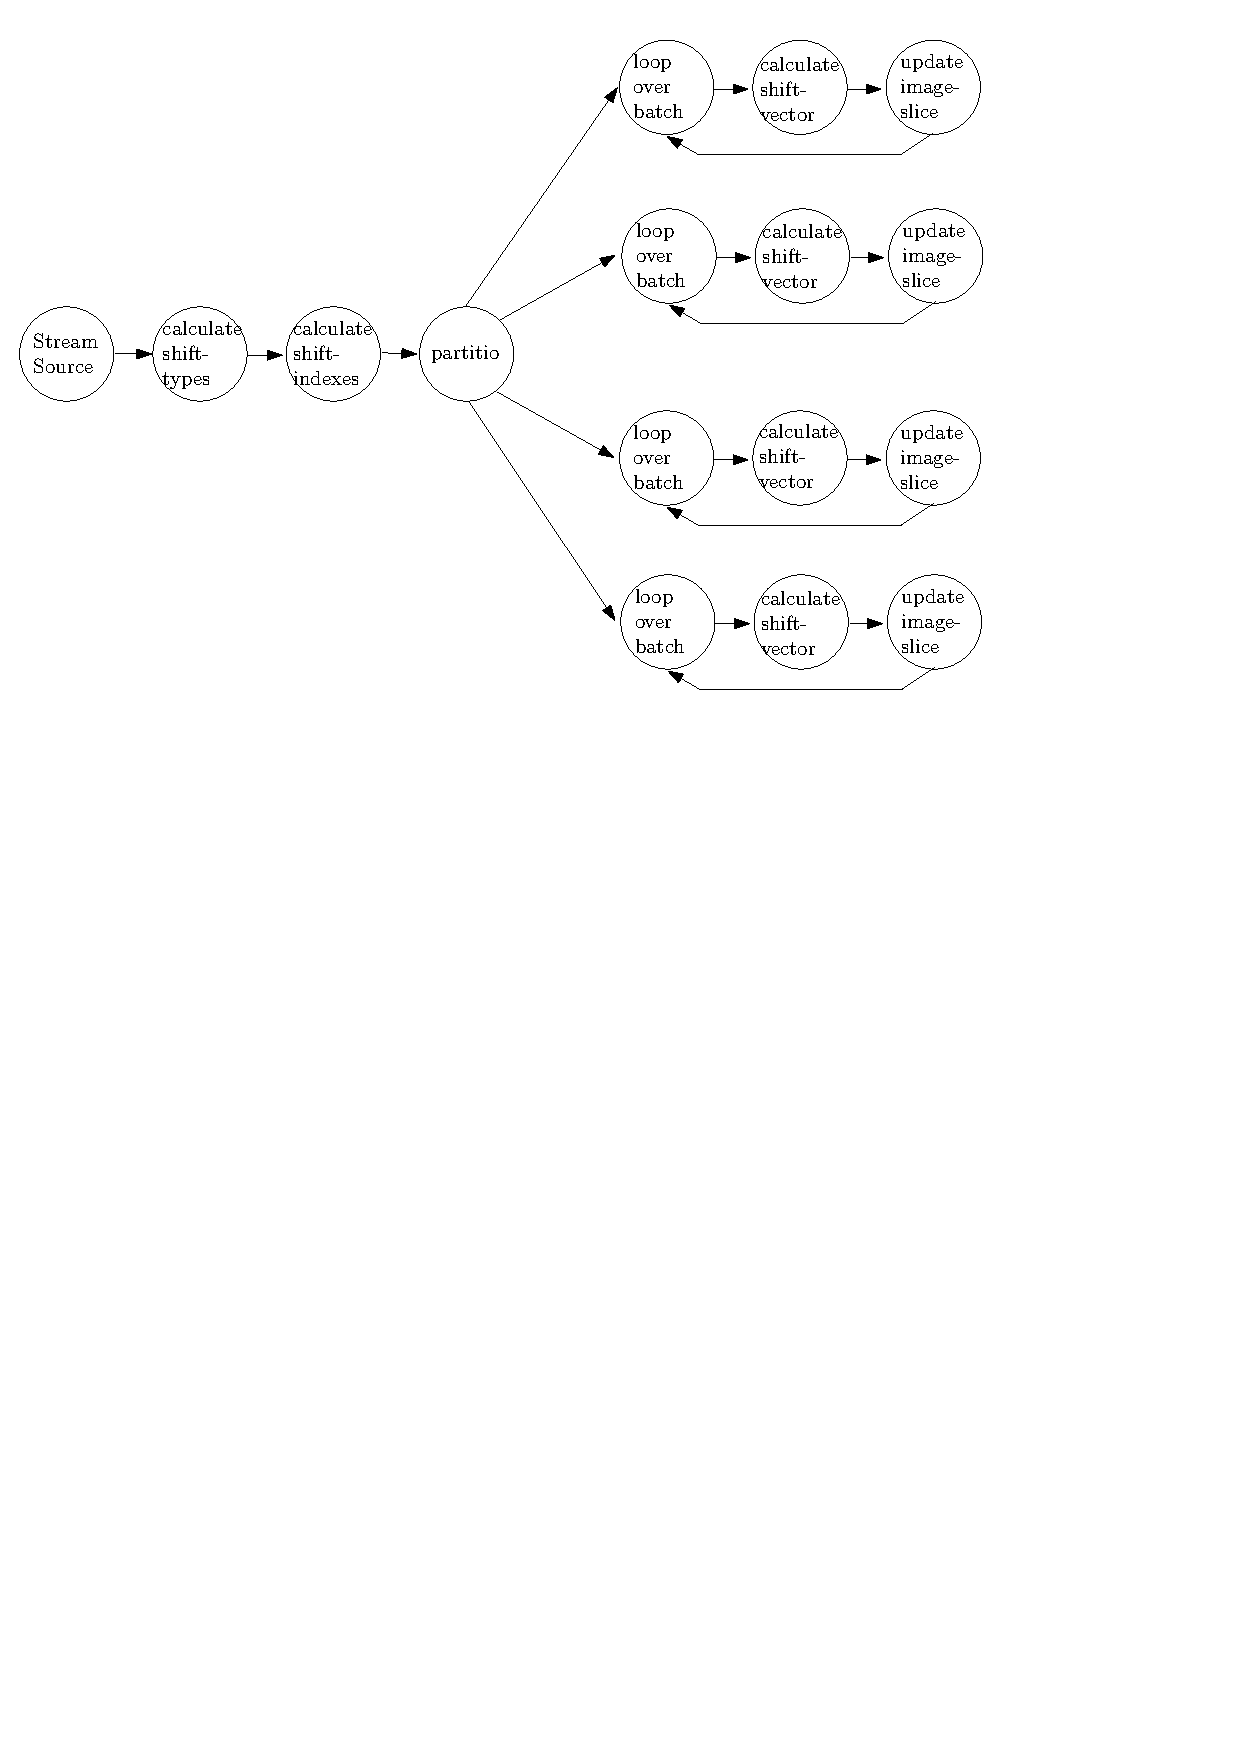
\includegraphics[width=400pt]{NAIVE_SPIFT_plan}
\end{center}
\caption{Flow chart of naive MPIFT using one master node that does initial calculation and passes it to $\phi=4$ processes}
\label{fig::naive_spift_plan}
\end{figure}

\subsubsection{MPIFT with Shift-Dictionary}
\label{sec::SPIFT_with_Dic}
Consider two visibilities in the same batch, $visibility_1$ and $visibility_2$. If they both have the same shift-type and shift-index, then we can add their shift-vectors together and handle it as one thing. This saves $\frac{N^2}{\phi}$ complex additions and costs $N$complex multiplications. If we consider that:
\[ \textrm{$\phi$ divides $N$ }
 \implies \phi\leq N \implies N\leq\frac{N^2}{\phi}.
 \]
  So combining the two visibilities is at leas as efficient as handling them separately.

The idea of shift-dictionaries is to create a row-shift-dictionary and a column-shift-dictionary. These dictionaries contain the $N$ combined shift-vectors for the $N$ shift-indices. Algorithm \ref{code::Spift_Shift_Dic} shows how to compute the shift-dictionary. \\

 Since communications-costs between different machines is high, it is inefficient to  compute the shift-vectors on the master-node and then send them to each process. But on a physical machine, processes can use shared memory, basically eliminating the communications-costs.
 
 The intuitive way to do this, is to divide the visbilities among the local processes, to ensure everyone does the same amount of work. But this could lead to a situation where two processes are handling two visibilities with the same shift-type and shift-index at the same time. They would both access the same part of the shift-dictionary at the same time, leading to simultaneous access and possible loss of data. This could be solved by locks, but this would increase the amount of computational overhead, and would defeat the purpose of every process taking the same amount of time, since processes would need to wait for memory access.
  
 Instead, we can order the visibilities by shift-type and shift-index in the master-node before sending them. This doesn't increase the communication-costs. Then we divide the possible shift-types and shift-indices among the processes, and have them each compute an equal part of the shift-dictionary. If the visibilities in the batch are well distributed, this would lead to an acceptable distribution of work. Figure \ref{fig::spift_with_dic_plan} shows the flow of creating the dictionaries and calculating MPIFT.\\
  
 The first entry-addition of a shift-vector into a shift-dictionary doesn't need to be added, all following ones do. So in the worst case, all visibilities have the same shift-type and shift-index. This would mean that one process has to calculate $N\cdot (\beta-1)$ complex additions and all $N$ complex multiplications. In the best case the visibilities are evenly distributed among the shift-types and -indices. This leads to $\frac{N}{\lambda}$ complex multiplications and $N\cdot \frac{\beta-N}{\lambda}$ complex additions. Since $\beta$ usually is large, the average case is much closer to the best case than to the worst case.

\begin{algorithm}
	\begin{algorithmic}[1]
		\State $dRow$ = \emph{new} dic
		\State $dCol$ = \emph{new} dic
		\For{ $(u_t, v_t, \vis_t)$ in ${visibilities}_t$}
			\State $isCS, si = $CalculatingShiftIndex($u_t,v_t$)
			\State $sv$ = ShiftVector($u_t,v_t,\vis_t,isCS$)
			\State $sv \leftarrow$ emptyvector$(N)$
			\For {$k \leftarrow 0$ \textbf{to} $N$}
				\If{ ($isCS$)}
					\State $sv[k] \leftarrow vis\cdot W^{(k\cdot u)\%N}$
				\Else
					\State $sv[k] \leftarrow vis\cdot W^{(k\cdot v)\%N}$
				\EndIf
			\EndFor
			\If {isCS}
				\If{$dCol$ contains $si$}
					\State $dCol[si] \leftarrow dCol[si]+sv$
				\Else
					\State $dCol[si] \leftarrow sv$
				\EndIf
			\Else
				\If{$rCol$ contains $si$}
					\State $rCol[si] \leftarrow rCol[si]+sv$
				\Else
					\State $rCol[si] \leftarrow sv$
				\EndIf
			\EndIf
		\EndFor
		\Return $({dRow}_t, {dCol}_t)$
	\end{algorithmic}
\caption{CalculatingShiftDictionary(${visibilities}_t, N$)}\label{euclid}
\label{code::Spift_Shift_Dic}
\end{algorithm}

\begin{figure}[H]
	\begin{center}
	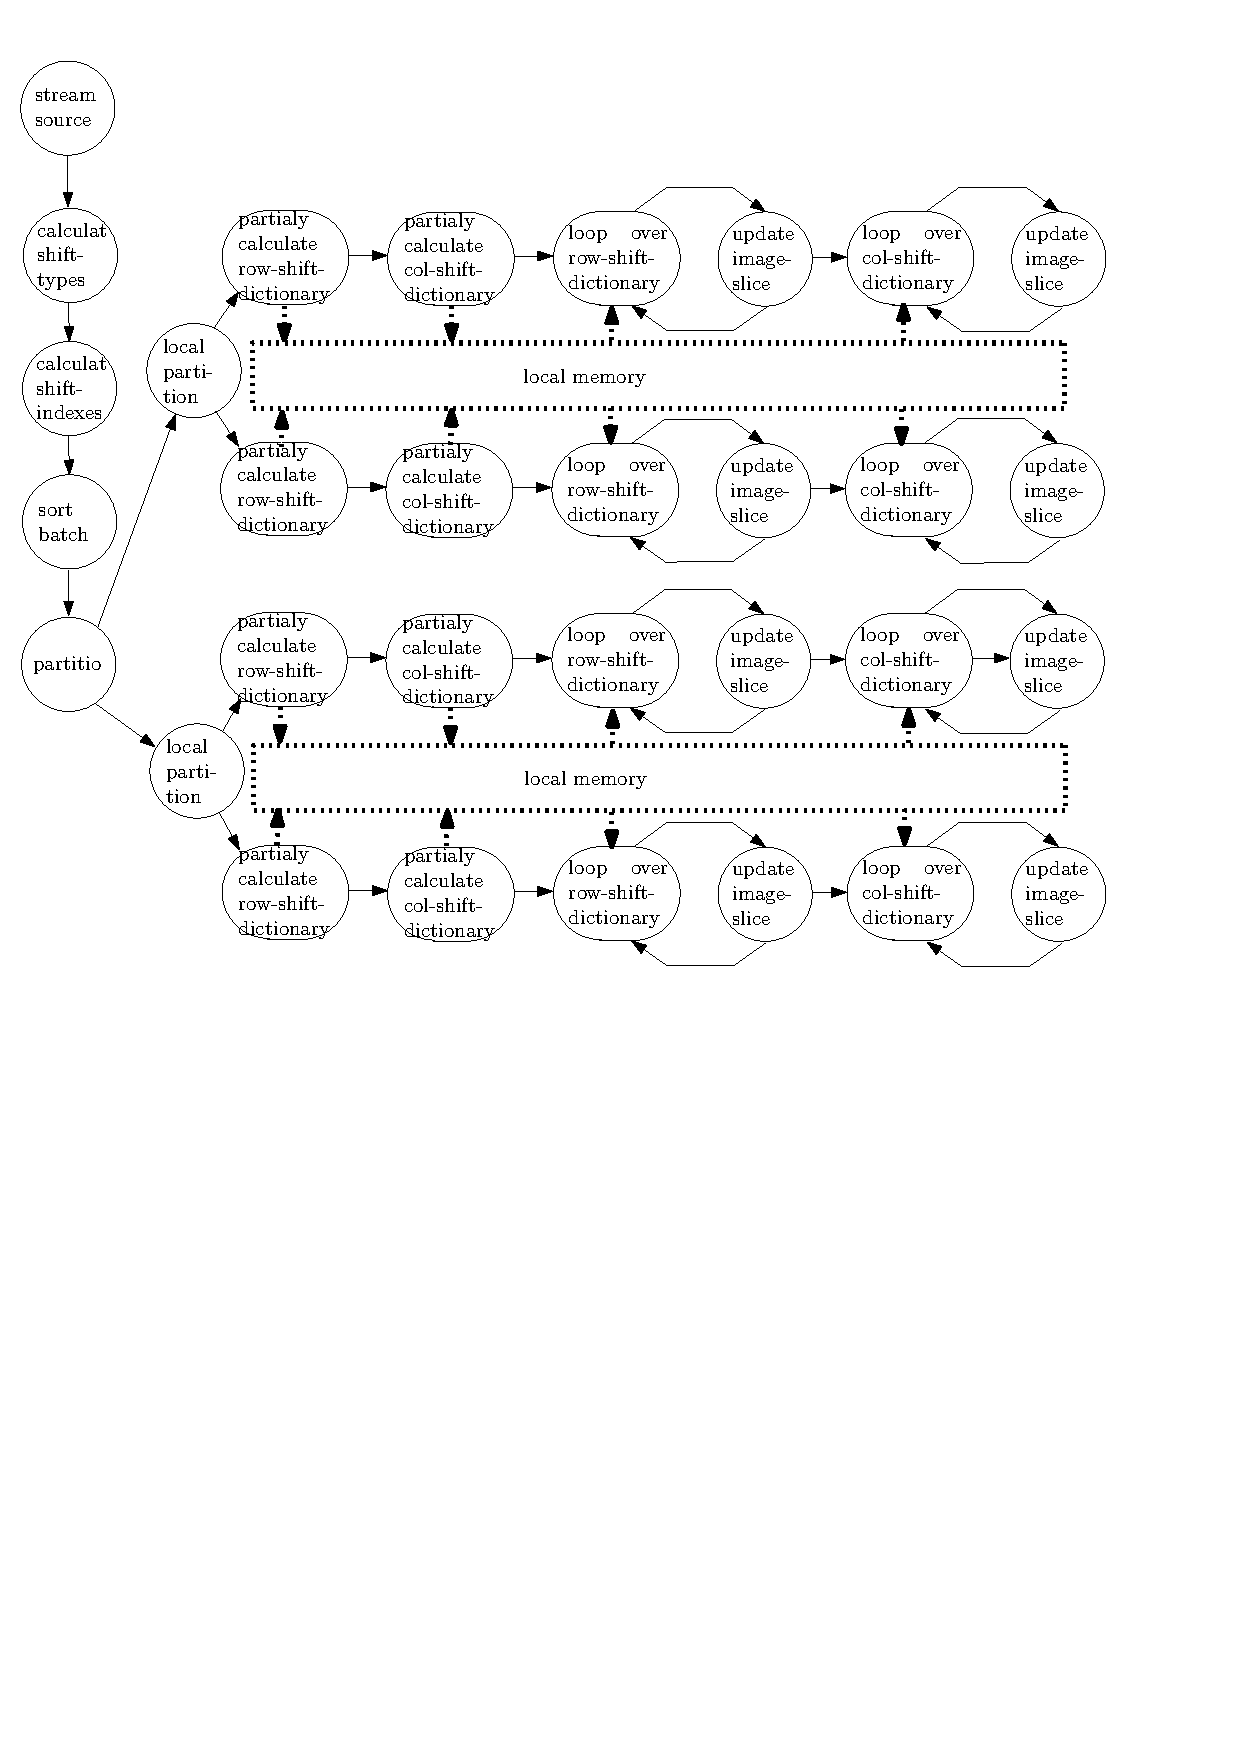
\includegraphics[width=400pt]{SPIFT_WITH_DIC_plan}
\end{center}
	\caption{Flow chart of MPIFT with shift-dictionaries. One master node does initial calculation and sorts the batch and passes it to $\omega=2$ machines running $\lambda=2$ processes each. Each machine has local memory that is shared between processes of that machine.}
	\label{fig::spift_with_dic_plan}
\end{figure}

\subsubsection{Example Shift-Dictionary}
\label{sec::exampleShiftDic}

In this section we will give a small example how to calculate a shift-dictionary. We will consider measurements on $N=4$ with an incoming batch of size $\beta = 12$, shown in Table \ref{fig::exampleBatch}. To keep it simple, we ignore that the visibilities would be sorted and handled by multiple processes.

\begin{figure} [h]
	\begin{center}
		\begin{tabular}{||c c c c c c c||} 
			\hline
			Number & $u$ & $v$ & $\vis$ & $isCS$ & shift-index & shift-vector\\ [0.5ex] 
			\hline\hline
			$1$ & $1$ & $2$ & $1+0i$ & true & 2 & (1+0i,0+1i,-1+0i,0-1i)\\
			\hline
			$2$ & $0$ & $2$ & $2+0i$ & false & 0 & (2+0i,-2+0i,2+0i,-2+0i)\\
			\hline
			$3$ & $2$ & $1$ & $3+0i$ & false & 2 & (3+0i,0+3i,-3+0i,0-3i)\\
			\hline
			$4$ & $0$ & $3$ & $0+4i$ & false & 0 & (0+4i,4+0i,0-4j,-4+0j) \\
			\hline
			$5$ & $3$ & $1$ & $5+0i$ & false & 3 & (5+0i,0+5i,-5+0i,0-5i)\\
			\hline
			$6$ & $1$ & $0$ & $0+6i$ & true & 0 & (0+6i,-6+0i,0-6i,6+0i) \\
			\hline
			$7$ & $3$ & $3$ & $7+7i$ & false & 1 & (7+7i,7-7i,-7-7i,-7+7i)\\
			\hline
			$8$ & $1$ & $1$ & $8+0i$ & false & 1 & (8+0i,0+8i,-8+0i,0-8i)\\
			\hline
			$9$ & $0$ & $3$ & $0+9i$ & false & 0 & (0+9i,9+0,0-9i,-9+0i)\\
			\hline
			$10$ & $2$ & $1$ & $10+10i$ & false & 2 & (10+10i,-10+10i,-10-10i,10-10i)\\
			\hline
			$11$ & $3$ & $3$ & $11+0i$ & false & 1 & (11+0i,0-11i,-11+0i,0+11i) \\
			\hline
			$12$ & $2$ & $0$ & $0+12i$ & true & 0 & (0+12i,0-12i,0+12i,0-12i)\\
			\hline
		\end{tabular}
	\end{center}
\captionof{table}[foo]{Example Batch for a $4\times 4$ image matrix}
\label{fig::exampleBatch}
\end{figure}

We first create an empty row-shift dictionary and an empty column-shift dictionary. The first three values can simply be added to them, since they differ in shift-index and shift-type. Table \ref{fig::shift_dic_after_3} shows what the shift-dictionaries would look like after this.

\begin{figure} [h]
	\begin{center}
		\begin{tabular}{||c c c c||} 
			\hline
			\multicolumn{4}{||c||}{column-shift-dictionary} \\
			\hline
			\hline
			 0  &  & 2 &    \\ [0.5ex] 
			\hline
			$-$ & & $1+0i$ & \\
			\hline
			$-$ & & $0+1i$ & \\
			\hline
			$-$ & & $-1+0i$ & \\
			\hline
			$-$ & & $0-1i$ " & \\
			\hline\hline
			\multicolumn{4}{||c||}{row-shift-dictionary} \\
			\hline
			\hline
			0 & 1 & 2 & 3 \\
			\hline
			$2+0i$ & $-$ & $3+0i$ & $-$ \\
			\hline
			$-2+0i$ & $-$ & $0+3i$ & $-$ \\
			\hline
			$2+0i$ & $-$ & $-3+0i$ & $-$ \\
			\hline
			$-2+0i$ & $-$ & $0-3i$ & $-$ \\
			\hline
		\end{tabular}
	\end{center}
\captionof{table}{Shift Dictionaries after first 3 visibilities from Table \ref{fig::exampleBatch} have been added}
\label{fig::shift_dic_after_3}
\end{figure}

The fourth visibility is row-shiftable and has a shift-index of 0. The dictionary already has an entry for this, so the shift-vector gets added to the existing one. This is shown in Table \ref{fig::shift_dic_after_4}. The other visibilities then get added in the same fashion. Table \ref{fig::shift_dic_after_all} shows what the shift-dictionary looks like after all 12 values have been added.

\begin{figure} [h]
	\begin{center}
		\begin{tabular}{||c c c c||} 
			\hline
			\multicolumn{4}{||c||}{column-shift-dictionary} \\
			\hline
			\hline
			 0 &   & 2 &     \\ [0.5ex] 
			\hline\hline
			 $-$ &  & $1+0i$ &\\
			\hline
			 $-$ &  & $0+1i$ &\\
			\hline
			 $-$ &  & $-1+0i$ &\\
			\hline
			 $-$ &  & $0-1i$ " &\\
			\hline\hline
			\multicolumn{4}{||c||}{row-shift-dictionary} \\
			\hline
			\hline
			 0 & 1 & 2 & 3 \\
			\hline
			 $2+4i$ & $-$ & $3+0i$ & $-$ \\
			\hline
			 $2+0i$ & $-$ & $0+3i$ & $-$ \\
			\hline
			 $2-4i$ & $-$ & $-3+0i$ & $-$ \\
			\hline
			 $-6+0i$ & $-$ & $0-3i$ & $-$ \\
			\hline
		\end{tabular}
	\end{center}
\captionof{table}{Shift Dictionaries after first four value from batch in Table \ref{fig::exampleBatch} was added to Table \ref{fig::shift_dic_after_3}}
\label{fig::shift_dic_after_4}
\end{figure}

\begin{figure} [H]
\begin{center}
	\begin{tabular}{||c c c c||} 
		\hline
		\multicolumn{4}{||c||}{column-shift-dictionary} \\
		\hline
		\hline
		 0 &  & 2 &    \\ [0.5ex] 
		\hline\hline
		 $0+18i$ &  & $1+0i$ &  \\
		\hline
		 $-6-12i$ &  & $0+1i$ &\\
		\hline
		 $0+6i$ &  & $-1+0i$ & \\
		\hline
		 $6-12i$ &  & $0-1i$ " & \\
		\hline\hline
		\multicolumn{4}{||c||}{row-shift-dictionary} \\
		\hline
		\hline
		 0 & 1 & 2 & 3 \\
		\hline
		 $2+13i$ & $26+7i$ & $13+10i$ & $5+0i$ \\
		\hline
		 $11+0i$ & $7-10i$ & $-10+13i$ & $0+5i$ \\
		\hline
		 $2-13i$ & $-26-7i$ & $-13-10i$ & $-5+0i$ \\
		\hline
		 $-15+0i$ & $-7+10i$ & $10-13i$ & $0-5i$ \\
		\hline
	\end{tabular}
\end{center}
\captionof{table}{Shift Dictionaries after adding all visibilities from Table \ref{fig::exampleBatch}}
\label{fig::shift_dic_after_all}
\end{figure}

\subsection{Doublestep}
\label{sec::DB}
Doublestep is an algorithm that we have developed to reduce the number of complex additions when updating the image matrix. In this section we will discuss how Doublestep works, not considering multiple processes. In Section \ref{sec::multiprocessingDoublestep} we will extend the algorithm to work with multiple processes and shared memory.

\subsubsection{Idea}
\label{sec::idea}

Consider two shift-vectors $\emph{a}_1$ and $\emph{a}_2$ with shift-index $s_1$ and $s_2$ where $s_2 = s_1+\frac{N}{2}$ which are both row-shiftable. In the first row, $\vec{a}_1$ and $\vec{a}_2$ are added 
\[
(\emph{a}_1^{0}+\emph{a}_2^{0}).
\] The superscript denotes by how much the vector is shifted. On the next row, we get 
\[
(\emph{a}_1^{s_1}+\emph{a}_2^{s_2}).
\]
 On the third row, it is 
\[
 \emph{a}_1^{2\cdot s_1}+\emph{a}_2^{2\cdot s_2} = \emph{a}_1^{2\cdot s_1}+\emph{a}_2^{2\cdot s_1+2\cdot \frac{N}{2}} = \emph{a}_1^{2\cdot s_1}+\emph{a}_2^{2\cdot s_1} = (\emph{a}_1^{0}+\emph{a}_2^{0})^{2\cdot s_1},
\]
  and on the forth
\[
  \emph{a}_1^{3\cdot s_1}+\emph{a}_2^{3\cdot s_2} = \emph{a}_1^{3\cdot s_1}+\emph{a}_2^{3\cdot s_1+\frac{N}{2}} = (\emph{a}_1^{s_1}+\emph{a}_2^{s_1 +\frac{N}{2}})^{2\cdot s_1}
\]
If we continue this line of thought, we get $(\emph{a}_1^{0}+\emph{a}_2^{0})^{4\cdot s_1}$ for the fifth and $(\emph{a}_1^{s_1}+\emph{a}_2^{s_1 +\frac{N}{2}})^{4\cdot s_1}$ for the sixth row.  \\

As we can see, we only need to perform two vector-additions, $\emph{a}_1^{0}+\emph{a}_2^{0}$ and $\emph{a}_1^{s_1}+\emph{a}_2^{s_2}$. These two rows form a $2\times N$-matrix. If we shift this matrix by a multiple of $2\cdot s_1$, it corresponds to the shifted addition of $\emph{a}_1$ and $\emph{a}_2$. We will call this matrix $\emph{m}_{2\cdot s_1}^2$, where the subscript denotes the shift-index of the shift-matrix, and the superscript denotes the number of rows. We can do this with all shift-vector-pairs to get $\frac{N}{2}$ shift-matrices, that all have an even shift-index.\\

Consider now two shift-matrices $m_s^2$ and $m_{s+\frac{N}{2}}^2$. In the first two rows of the image matrix the two matrices are added together:
\[
(m_s^{2,0}+m_{s+\frac{N}{2}}^{2,0}).
\] The second superfix denotes the shift. In the third and fourth row, they both get shifted by $s$ and $s+\frac{N}{2}$ respectively 
\[
(m_s^ {2,s}+m_{s+\frac{N}{2}}^{2, s+\frac{N}{2}}).
\]
The fifth and sixth row are again just the result from the first two rows, shifted by $2\cdot s$,
\[ 
(m_s^ {2,2\cdot s}+m_{s+\frac{N}{2}}^{2, 2\cdot s+2\cdot \frac{N}{2}})=(m_s^{2,0}+m_{s+\frac{N}{2}}^{2,0})^{2\cdot s}.
\]
Similarly, the seventh and eight row are simply the third and fourth, shifted by $2\cdot s$,
\[ \big(m_s^ {2,3\cdot s}+m_{s+\frac{N}{2}}^{2, 3\cdot s+3\cdot \frac{N}{2}}\big)=\big(m_s^{2,s}+m_{s+\frac{N}{2}}^{2,s+\frac{N}{2}}\big)^{2\cdot s}.
\]
As we see, we can use the same method as before to calculate $4\times N$ shift-matrices. We then use the same method to calculate the shift-matrices of size $8 \times N$. We call the calculation of a new set of shift-matrices a step of Doublestep.
 
In the \emph{i-th} step of Doublestep, we calculate $2^{n-i}$ matrices of size $k\times N$, $k=2^i$. Since the shift-matrices of step \emph{i} must have shift-indices that are twice the shift-index of a matrix of step \emph{i-1}, all shift-matrices of step \emph{i} are multiples of k. The shift-matrices of the step $i$ can be calculated with using equation \eqref{calc::formulaShiftMatrix}, where $k=2^i$ and s is a multiple of k that is smaller than N. $\times$ denotes the concatenation of two matrices.
Figure \ref{fig::doubleStepVisualized} shows how shift-matrices combine to make shift-matrices of a higher degree.\\

\begin{equation} [h]
\emph{m}_{s}^k=(\emph{m}_{\frac{s}{2}}^{\frac{k}{2},0}+\emph{m}_{\frac{s+N}{2}}^{\frac{k}{2},0})\times (\emph{m}_{\frac{s}{2}}^{\frac{k}{2},\frac{s}{2}}+\emph{m}_{\frac{s+N}{2}}^{\frac{k}{2},\frac{s+N}{2}})
\label{calc::formulaShiftMatrix}
\end{equation}

\begin{figure}[ht!]
	\begin{center}
	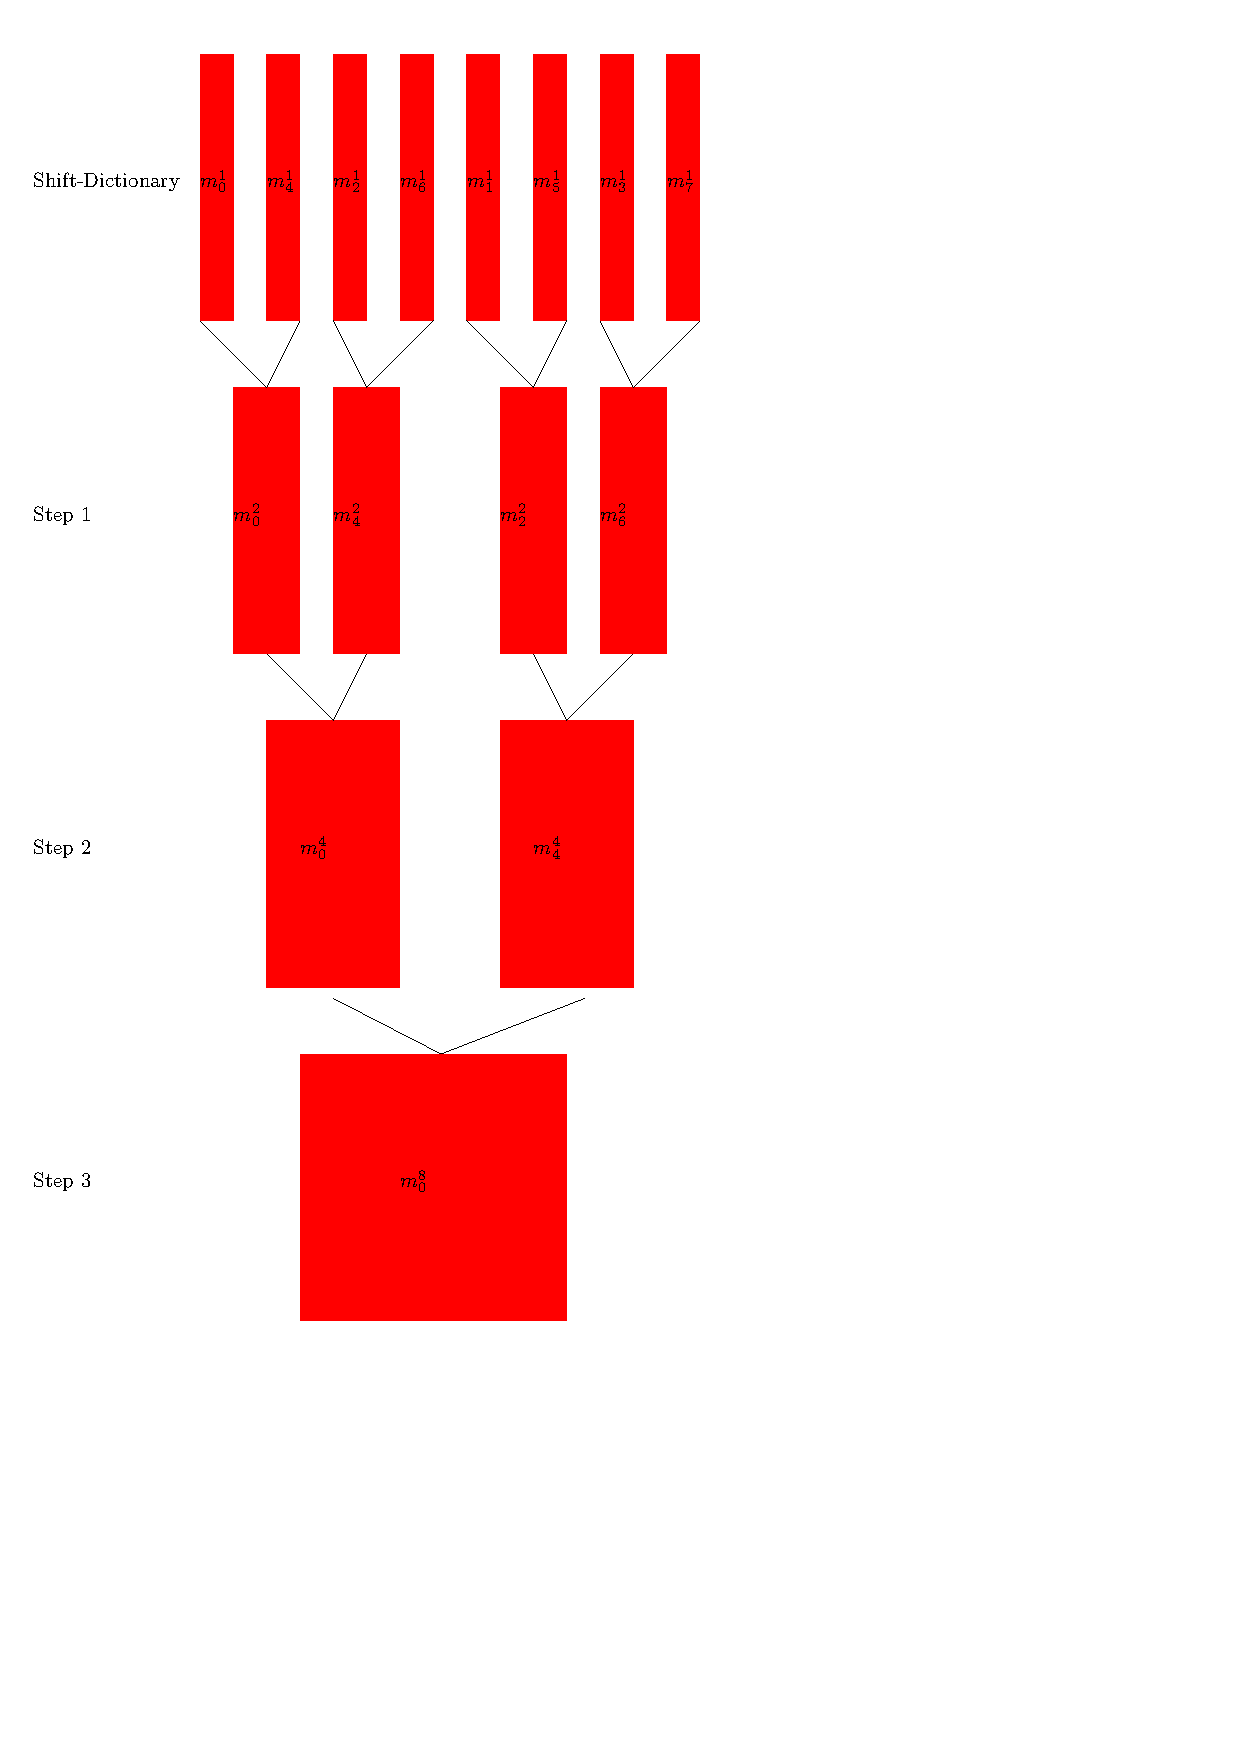
\includegraphics[height=\textheight-3cm]{Doublestep_overview}
\end{center}
	\caption{Illustration on how Doublestep combines smaller shift-matrices to build bigger ones for column-shift and $N=8$}
	\label{fig::doubleStepVisualized}
\end{figure}

At the $n^{th}$ step of Doublestep, we get just one $N\times N$ matrix with shift-index 0, $m_0^N$. Adding this matrix to the old image-matrix is equivalent to updating it with all visibilities from the batch.

\subsubsection{MPIFT with dictionaries and Doublestep algorithm}
\label{sec::algorithm}

Algorithm \ref{code::DS_Doublestep} performs MPIFT with dictionaries and Doublestep, which consists of three phases. In the first phase, the shift-dictionary is calculated. This happens in the same way as in the MPIFT with dictionary algorithm (Algorithm \ref{code::Spift_Shift_Dic}). In the second phase, the steps of Doublestep are performed for row- and column-shifts, to calculate the two shift-matrices $m_{0, row}^N$ and $m_{0,col}^N$. This is shown in Algorithm \ref{code::DS_StepsOfDoublestep}. In the third and final step, the two shift-matrices are added to the existing image matrix.



\begin{algorithm}
	\begin{algorithmic}[1]
		\State $dRow_t, dCol = CalculatingShiftDictionary(visibilities_t,N)$
		\State $(m_{0,row}^N,m_{0,col}^N) = Doublestep({dRow}_t,{dCol}_t, N)$
		\State $I_{t+1} \leftarrow I_t + m_{0,row}^N + m_{0,col}^N$
		\State \Return $I_{t+1}$
	\end{algorithmic}
\caption{MPIFTwithDictionariesAndDoublestep(${visibilities}_t, N, I_t$)}\label{euclid}
\label{code::DS_Doublestep}
\end{algorithm}


\begin{algorithm}
	\begin{algorithmic}[1]
		\For{i $\leftarrow 0$ to $N$}
			\State $m_{i,row}^{1} = dRow[i]$
			\State $m_{i,col}^{1} = dCol[i]$
		\EndFor
		\For{ $i\leftarrow 1$ to $\log(N)$}
			\State $k = 2^i$
			\For{$s \leftarrow 0,k,2k$ to $N-k$}
				\State $m_{s,row}^k \leftarrow (m_{\frac{s}{2},row}^{\frac{k}{2},0}+
				m_{\frac{s+N}{2},row}^{\frac{k}{2},0})
				\times
				(m_{\frac{s}{2},row}^{\frac{k}{2},\frac{s}{2}}+
				m_{\frac{s+N}{2},row}^{\frac{k}{2},\frac{s+N}{2}})
				$
				\State $m_{s,col}^k \leftarrow (m_{\frac{s}{2},col}^{\frac{k}{2},0}+
				m_{\frac{s+N}{2},col}^{\frac{k}{2},0})
				\times
				(m_{\frac{s}{2},col}^{\frac{k}{2},\frac{s}{2}}+
				m_{\frac{s+N}{2},col}^{\frac{k}{2},\frac{s+N}{2}})
				$
			\EndFor
		\EndFor
		\Return $(m_{0,row}^N,m_{0,col}^N)$
	\end{algorithmic}
\caption{Doublestep(${dRow}_t,{dCol}_t, N$)}\label{euclid}
\label{code::DS_StepsOfDoublestep}
\end{algorithm}

\subsubsection{Complexity}
\label{sec::DB_complexity}

Calculating a single shift-vector implies $N$ complex multiplications. This means that $N\cdot \beta$ complex multiplications are required for the full shift-dictionary. The first shift-vector for each shift-index does not need to be added to anything. But each subsequent shift-vector with the same shift-index must be added to the existing one. Each vector-addition needs $N$ complex additions. So, in the best case, there is a visibility for every shift-index, and $N\cdot (\beta - \frac{3N}{2})$ complex additions are required. In the worst case, all visibilities have the same shift-index, and $N\cdot (\beta - 1)$ complex additions are required. With large buffer-size, it does not matter and we can approximate and say it requires $N\cdot \beta$ complex additions. \\

In each step of Doublestep, $\frac{N}{2^i}=\frac{N}{k}$ shift-matrices of size $k\times$ or $N\times k$ if we are handling column-shift need to be calculated. Each requires $k\cdot N$ complex additions, so one step requires 
\[
k\cdot N\cdot \frac{N}{k}=N^2
\]
complex additions.

Doublestep has $n$ steps for row- and $n$ steps for column shift. In total, we therefore get
\[
2\cdot n\cdot N^2=2\cdot \log(N)\cdot N^2
\]
complex additions\\

The two final shift-matrices $m_0^N$ for row- and column-shift are added to the existing image-matrix. Both have size $N\times N$. Accordingly, $2\cdot N^2$ complex additions are required for this step.\\

Complex multiplications only appear in the calculation of the shift-dictionary. Consequently 
\[
N\cdot \beta
\] complex additions are required. Complex additions are required in for the shift-dictionary and Doublestep.
\[
N\cdot \beta + 2\cdot \log(N)\cdot N^2+2\cdot N^2
\] complex additions are therefore approximately needed to perform MPIFT with dictionaries and Doublestep, which means it has an asymptotic complexity of
\[
\mathcal{O}(N \beta)
\] complex additions and
\[
 \mathcal{O}({N \beta + N^2 \log(N)})
\]
complex additions.


\subsubsection{Example}
\label{sec::DS_example}

This section shows an example of how Doublestep works. We will continue using the example for Sections \ref{sec::exampleShiftDic}, and compute Doublestep on the row-shift-dictionary from Figure \ref{fig::spift_with_dic_plan}. From that section we know that $N=4$. Since the row-shift-dictionary is already computed, we already have all shift-matrices of size $1\times 4$. Each matrix corresponds to the entry in the shift-dictionary with the same shift-index, as shown in Figure \ref{calc::doublestepEx0}. 

\begin{figure} [H]
	\begin{align*} 
	m_0^1&=\begin{pmatrix}
	(2+13i) & (11+0i) & (2-13i) & (-15+0i)
\end{pmatrix} \\
m_1^1&=\begin{pmatrix}
	(26+7i) & (7-10i) & (-26-7i) & (-7+10i)
\end{pmatrix} \\
m_2^1&=\begin{pmatrix}
	(13+10i) & (-10-13i) & (-13-10i) & (10-13i)
\end{pmatrix} \\
m_1^1&=\begin{pmatrix}
	(5+0i) & (0+5i) & (-5+0i) & (0-5i)
\end{pmatrix}
	\end{align*}
	\caption{Doublestep example step 0}
	\label{calc::doublestepEx0}
\end{figure}

Since $N=4$, we know that $n=2$, so we need to compute $2$ steps. First, we will calculate $m_0^2$ and $m_2^2$. To calculate $m_0^2$, we need 
\[
m_{\frac{0}{2}}^{\frac{2}{2}}=m_0^1 \textrm{ and } m_{\frac{0+4}{2}\%4}^{\frac{2}{2}}=m_2^1.
\]
The first row of $m_0^2$ is $m_0^1$ and $m_0^2$ added together without any shift. For the next row, both $m_0^1$ and $m_2^1$ are shifted by their shift index. In the case of $m_0^1$ this means that it is shifted by $0$, i.e. not actually shifted.

For $m_2^2$ we need 
\[
m_{\frac{2}{2}}^{\frac{2}{2}}=m_1^1 \textrm{ and } m_{\frac{2+4}{2}\%4}^{\frac{2}{2}}=m_3^1.
\]
Again, the first row is just the two rows without any shift happening. In the second row both vectors get shifted by their shift-index, so $1$ and $3$. The result can be seen in Figure \ref{calc::doublestepEx1}.

Note that the rule is not, that the first row is not shifted, and the second is. For a shift-matrix $m_i^d$, the first $\frac{d}{2}$ rows are not shifted. In step one this is just be one row.

\begin{figure} [H]
	\begin{align*}
	m_0^2&=\begin{pmatrix}
	(15+23i) & (1-13i) & (-11-23i) & (-5-13i) \\
	(-11-3i) & (22-13i) & (15-3i) & (-25-13i)
	\end{pmatrix} \\
	m_2^2&=\begin{pmatrix}
	(31+7i) & (7-5i) & (-31-7i) & (-7-5i) \\
	(-7+15i) & (21+7i) & (7-15i) & (-21-7i)
	\end{pmatrix} \\
	\end{align*}
	\caption{Doublestep example step 1}
	\label{calc::doublestepEx1}
\end{figure}

In step 2 we calculate one shift-matrix $m_0^4$. It is composed of
\[
m_{\frac{0}{2}}^{\frac{4}{2}}=m_0^2 \textrm{ and }
m_{\frac{0+4}{2}\%4}^{\frac{4}{2}}=m_2^2.
\]
For the first two rows, we just add the values of $m_0^2$ and $m_2^2$. For the third and fourth row, we shift $m_0^2$ by 0 (which is again the same as not shifting), and $m_2^2$ by 2, before adding them together. This is shown in Figure \ref{calc::doublestepEx2}. Thus we have calculated the final shift-matrix. Adding this to the existing image-matrix will be equivalent to performing SPIFT on all twelve visibilities of Table \ref{fig::exampleBatch}.


\begin{figure} [H]
	\begin{center}
$m_0^4=\begin{pmatrix}
(46+30i) & (8-18i) & (-42-30i) & (-12-18i) \\
(-18+12i) & (43-6i) & (22-18i) & (-46-20i) \\
(16+16i) & (-6-18i) & (20-16i) & (2-18i) \\
(-4-18i) & (1-20i) & (8+12i) & (-4-6i)
\end{pmatrix}$
	\end{center}
\caption{Doublestep example step 2}
\label{calc::doublestepEx2}
\end{figure}


\subsection{Multiprocessing MPIFT with dictionaries and Doublestep}
\label{sec::multiprocessingDoublestep}

In Section \ref{sec::DB} we only used one process. MPIFT can be improved by using multiple processes to calculate the shift-dictionaries and Doublestep. For the processes to cooperate in performing Doublestep, they need to share a lot of data. In practice, this is only feasible if the processes run on the same physical machine, otherwise the communication costs become too large.
When performing MPIFT with dictionaries and Doublestep in parallel, we divide the image matrix into sub-grids. Unlike naive MPIFT, not every process gets its own sub-matrix. Rather, all processes on the same machine work together to calculate one sub-matrix. So, we end up with $\omega$ sub-matrices. Figure \ref{fig::doublestep_plan} shows the flow of MPIFT with dictionaries and Doublestep.\\

	When slicing the image-matrix into sub-matrices, we can either slice with the rows or with the columns. If we slice with the rows we get sub-matrices of size $D\times N$, if we slice with columns they are of size $N\times D$, where $D=\frac{N}{\omega}$. The choice is arbitrary. In this report, we assume that we sliced with the rows.\\

After having decided if we splice with rows or columns, some vector-shifts will go with the slice, and others against it. Here the row-shift goes with and column shift against the slice. This has ramifications on how Doublestep is performed. We need to compute row-Doublestep, differently then column-Doublestep. \\

\begin{figure}[H]
	\begin{center}
	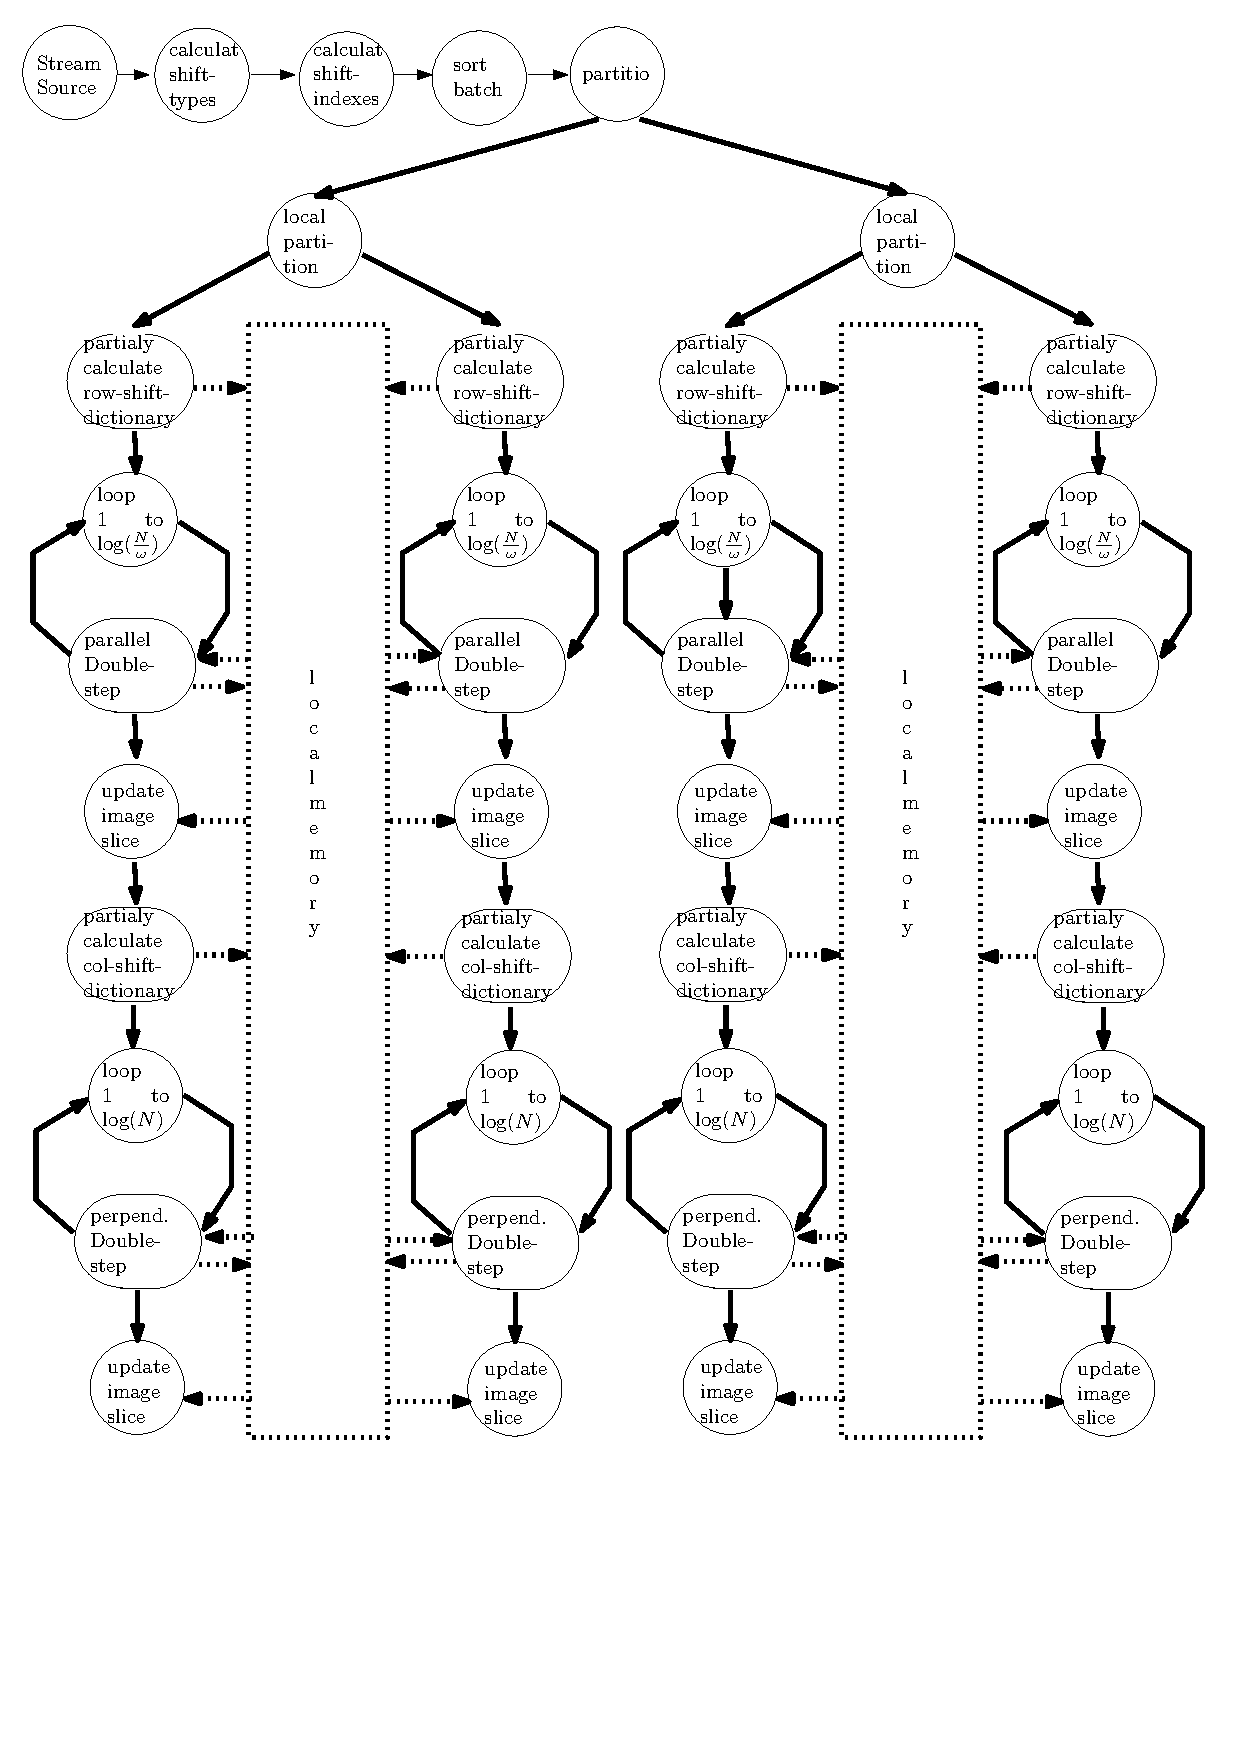
\includegraphics[width=370pt]{DOUBLESTEP_plan}
\end{center}
	\caption{Flow chart of MPIFT with dictionaries and Doublestep. One master node does initial calculations, sorts the batch and passes it to $\omega=2$ machines running $\lambda=2$ processes each. Each machine has local memory that is shared between processes of that machine.}
	\label{fig::doublestep_plan}
\end{figure}

\subsubsection{MPIFT with dictionaries and row-Doublestep}
\label{sec::parallelDoublestep}

In the row-shift case, a machine first receives a dictionary containing all visibilities with row-shift, organized by shift-index.
Since all row-shift-vectors are needed in every slice, each machine needs to calculate the full shift-dictionary first. All processes can work together on this, using shared memory.
This is done the same way as in Section \ref{sec::SPIFT_with_Dic}.\\

$N$ shift-vectors need to be calculated and each machine has $\lambda$ local processes to do so. Each process has to calculate $r$ row-shift-vectors and store them in the row-shift-dictionary, where $r=\frac{N}{\lambda}$. Since $N>\lambda$ and both $N$ and $\lambda$ are powers of two, this is always possible. Each process can look up the visibilities it needs to calculate its shift-vectors. Since it is possible that a shift-index has more visibilities associated with it, some processes will take longer than others. The processes cannot work together to share the work more evenly, because this would mean that multiple process must write to the same part of memory in the shift-dictionary, leading to multithreading problems.\\


After having calculated the row-shift-dictionary, row- Doublestep needs to be performed. Since in the end, only a $D\times N$, with $D=\frac{N}{\omega}$, slice of the image-matrix needs to be calculated, it is more efficient to only use Doublestep until a shift-matrix size of $D\times N$ is reached. Since $N$ and $\beta$ are powers of two, there will always be a set of shift-matrices with exactly this size. They are the shift-matrices $m_{i\cdot D}^{D}$, with $i\in \{0,1,...,\frac{N}{D}-1 \}$.

The processes can calculate each step of Doublestep together. Since every row of every shift-matrix is only dependent of the shift-matrices of the previous step, we can just distribute all the rows of all the shift-matrices that need to be calculated in each step evenly among all processes. This means that early on a process will calculate one or multiple shift-matrices alone. In later steps, the rows of a single shift-matrix will be calculated by different processes. Figure \ref{fig::rowDSprocesses} shows how the shift-matrices calculation of row-Doublestep would be divided among four processes. As we see in the last step multiple processes calculate one shift-matrix together. \\
 
 \begin{figure}[H]
 	\begin{center}
 		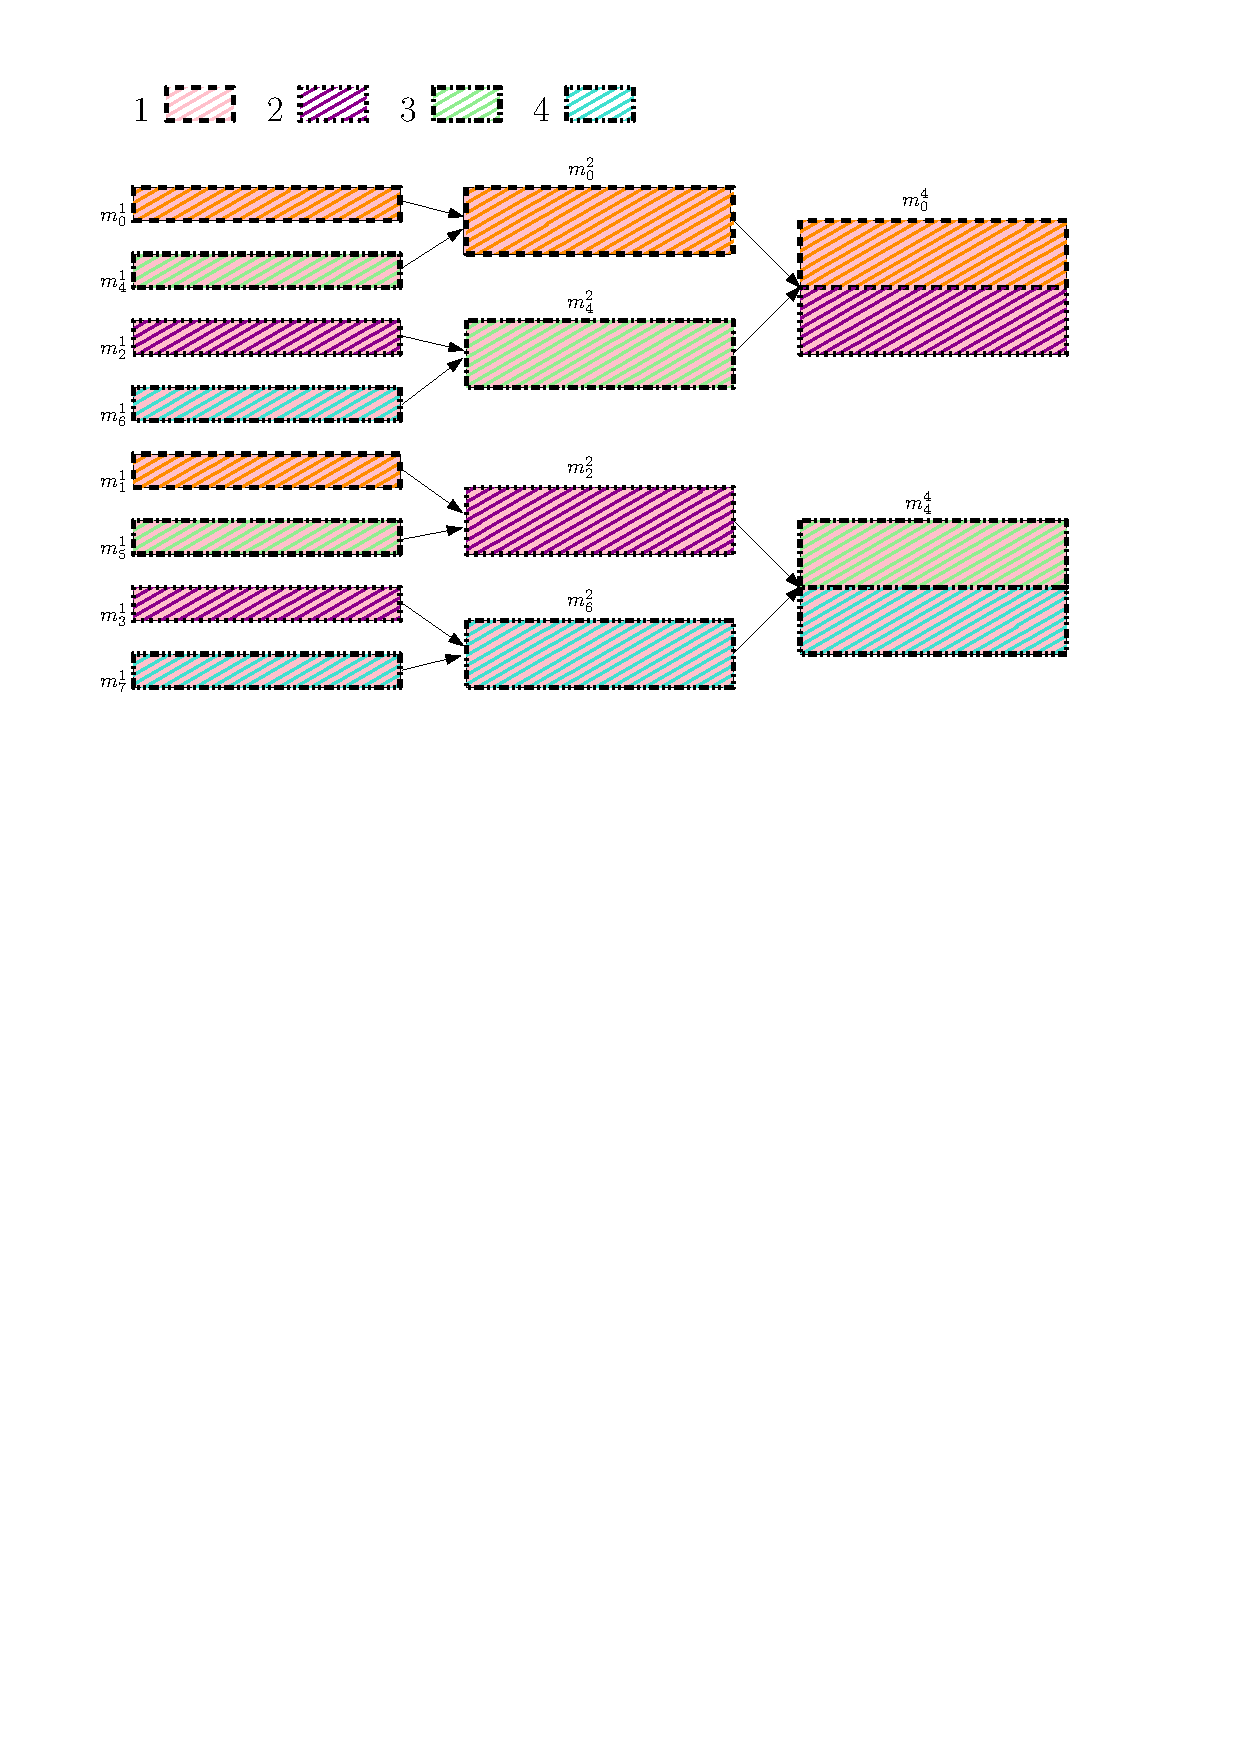
\includegraphics[width=400pt]{processes_colum_doublestep}
 		\caption{Calculation of row-dictionary and row-Doublestep performed by 4 processes. The color in each step shows, which section gets performed by which process. $N=8$, $\omega = 2$, $\lambda=4$.}
 		\label{fig::rowDSprocesses}
 	\end{center}
 \end{figure}
 
In the end, the shift-matrices $m_{i\cdot D}^{D}$ need to be added to the image-matrix-slice. The rows of the slice can be distributed evenly to the processes, so each updates the same number of rows. When adding the values of $m_{i\cdot D}^{D}$ to the slice, each shift-matrix needs to be shifted by $rank\cdot (i\cdot D)$, where $rank$ is the rank of the machine that is hosting the sub-matrix-slice.\\

Figure \ref{fig::rowDSprocesses} shows how $\lambda=4$ processes calculate row-Doublestep together on one of two machines $\omega=2$.

Before they can start with Doublestep, they need to construct the row-shift-dictionary together. Every process has a list of all visibilities. Process one calculates all shift-vector for visibilities with shift-index zero and build their combined shift-vector. It then stores it into shared machine-memory, that is accessible by all processes. It then does the same for shift-index one. The second process calculates the shift-dictionary entries for shift-indices two and three. Process three does shift-indices four and five, and process four calculates for shift-index six and seven. These corresponds to the colored $1 \times N$-sections in Figure \ref{fig::rowDSprocesses}.

Once all processes have calculated their part of the dictionary and stored it into shared machine-memory, they can calculate the first step of row-Doublestep. Since four shift-matrices need to be calculated and the machine is using four processes, every process calculates exactly one shift-matrix. Process one calculates $m_0^2$. To do so, it needs to read two entries from the shift-dictionary, $m_0^1$ and $m_4^1$. Since both have been written to shared machine-memory, process one can access them both. Process adds $m_0^1$ and $m_4^1$ together to form the first row of $m_0^2$. It then shifts $m_0^1$ and $m_4^1$ by their shift-index before adding them together again to get the second row of $m_0^2$. 
It then writes $m_0^4$ to shared machine-memory. Process two does the same for $m_4^2$. Process two was not involved in calculating the shift-dictionary entries it need $m_2^1$ and $m_6^1$. This does not matter, since the whole shift-dictionary is stored in shared machine-memory, so process two can read them. Process three calculates and stores $m_2^2$ and process four $m_6^2$.

In the second step, there are more processes then shift-matrices. So multiple processes have to calculate one matrix. Process one and two calculate shift-matrix $m_0^4$ together. Process one will calculate the first two rows and process two the second two. Both will need access to $m_0^2$ and $m_4^2$. Since both these shift-matrices are stored in shared machine-memory, both processes can access them. And since they only need to read the values, they can access them simultaneously. Process one adds together $m_0^4$ and $m_4^4$ to geth the first two rows of $m_0^4$. Process two shifts $m_0^4$ and $m_4^4$ by their shift-index before adding them together to get the third and fourth row of $m_0^4$. They both write there results to the same shift-matrix $m_0^4$ in shared machine-memory. Since they write to different sections, there is no danger in them accessing the shift-matrix simultaneously, as long as an architecture has been chosen, that allows the change of one value without affecting the other ones. Processes three and four calculate the shift-matrix $m_4^4$ in the same fashion, by accessing $m_2^2$ and $m_6^2$ from shared machine-memory.

The amount of machines used in this example is $\omega=2$. Row-Doublestep only needs to be performed, until we get shift-matrices of size $\frac{N}{\omega}\times N=\frac{N}{2}\times N$. Since this is reached after step two of row-Doublestep, there is no third step. Both shift matrices $m_0^4$ and $m_4^4$ can now be used to update the image-matrix.

\subsubsection{MPIFT with dictionaries and column-Doublestep}
\label{sec::perpendicDoublestep}

When we consider column-shift, we see that not every row of each shift-matrix will appear in the final image-slice. Take for example the column-shift-matrix $m_{0}^4$. Since it has shift-index $0$, only the rows that correspond to the image-slice being calculated appear in the final image-slice. Figure \ref{fig::recursiveLines} shows which lines would be needed to calculate the sub-matrix of a $8\times 8$ image-matrix by machine 2 of $\omega=2$.

\begin{figure}[ht!]
	\begin{center}
	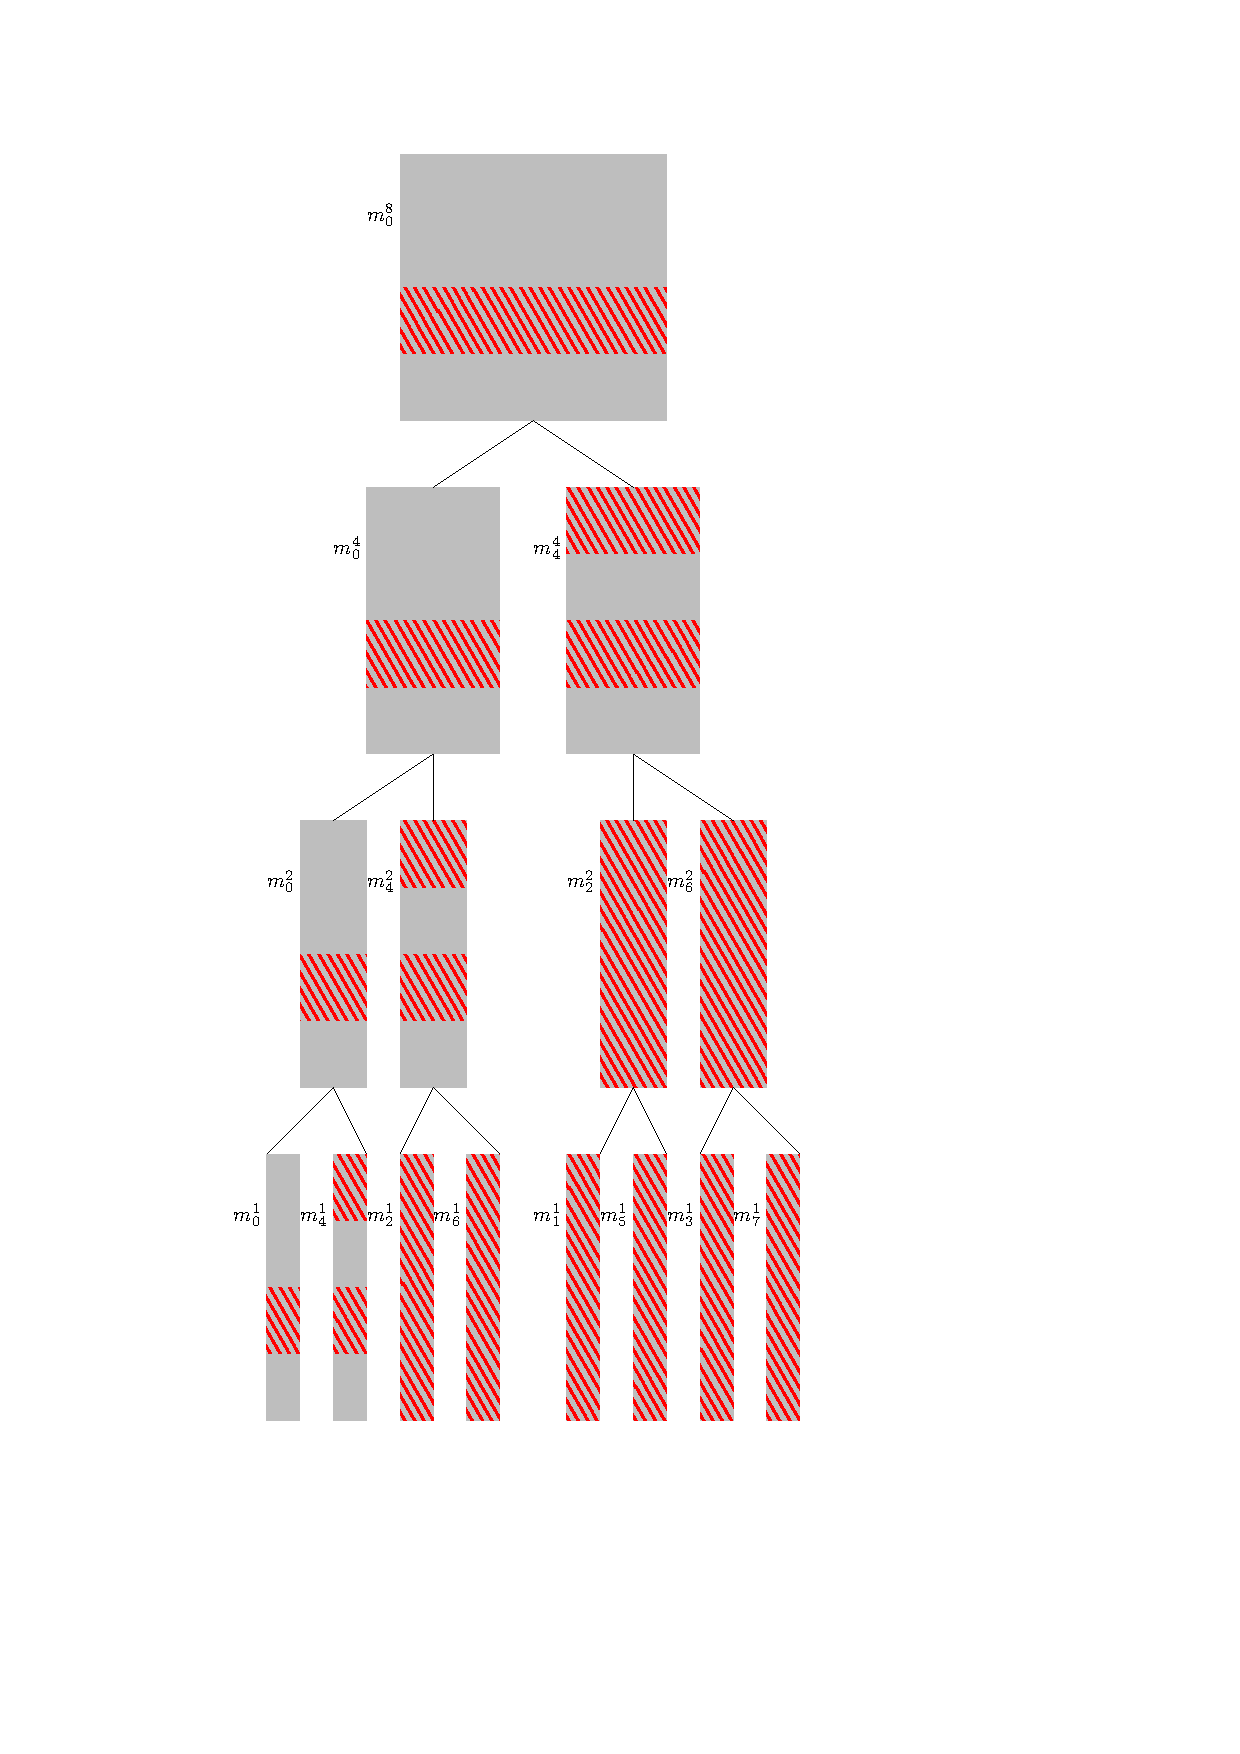
\includegraphics[height=\textheight-3cm]{Recursive_lines}
	\caption{Required Lines for column-Doublestep. $N=8$, $\omega = 4$, $rank=2$. Red marks the lines that need to be calculated for each shift-matrix.}
	\label{fig::recursiveLines}
\end{center}
\end{figure}

Before we calculate Perpendicular Doublestep, we need to find out, which rows of which shift-matrices are even needed. An intuitive way of doing this, is to look what lines are needed from $m_0^N$, and calculate recursively, what lines are needed on shift-matrices of earlier steps to compute this matrix. This can be seen in Algorithm \ref{code::DS_Per_Lines_Rec}. Note that in reality, an iterative approach tends to be faster, than a recursive one.\\


\begin{algorithm}
	\begin{algorithmic}[1]
		\If {D = 1}
			\State \Return \{(D,lines)\}
		\EndIf
		\State neededLns = \{\}
		\For{$(l,si)$ in $lines$}
			\State neededLns $\leftarrow neededLns \cup \{(l,\frac{si}{2}),((l+\frac{si}{2})\%N,\frac{si}{2})\}$
			\State neededLns $\leftarrow neededLns \cup \{(l,\frac{si+N}{2}\%N),((l+\frac{si+N}{2})\%N,\frac{si+N}{2}\%N)\}$	
		\EndFor
		\State \Return $\{(D,lines)\} \cup NeededLinesPerpendicularRec(N,\frac{D}{2},neededLns)$
	\end{algorithmic}
\caption{NeededLinesColumnDoublestepRec($N,D,lines$)}\label{euclid}
\label{code::DS_Per_Lines_Rec}
\end{algorithm}


The recursive functions calculated the lines needed from every shift-matrix. Since the shift-matrices of size $N\times1$ are the entries of the shift-matrix, we can use this to only calculate the parts of each shift-vector that are actually needed, saving some complex operations.

Then the processes can go on and calculate the steps of Doublestep. Since different matrices will have different amounts of required lines, we cannot just distribute the shift-matrices in each step to different processes. Instead, we evenly distribute the set of all required lines among the processes. Each line of each shift-matrix is only dependent on the shift-matrices in the previous step, so there are no problems with simultaneous write access. Algorithm \ref{code::DS_Per} implements column-Doublestep computation. Figure \ref{fig::colum_DS_distribution} shows an example of how  the lines to calculate are divided among processes.

\begin{figure}[ht!]
	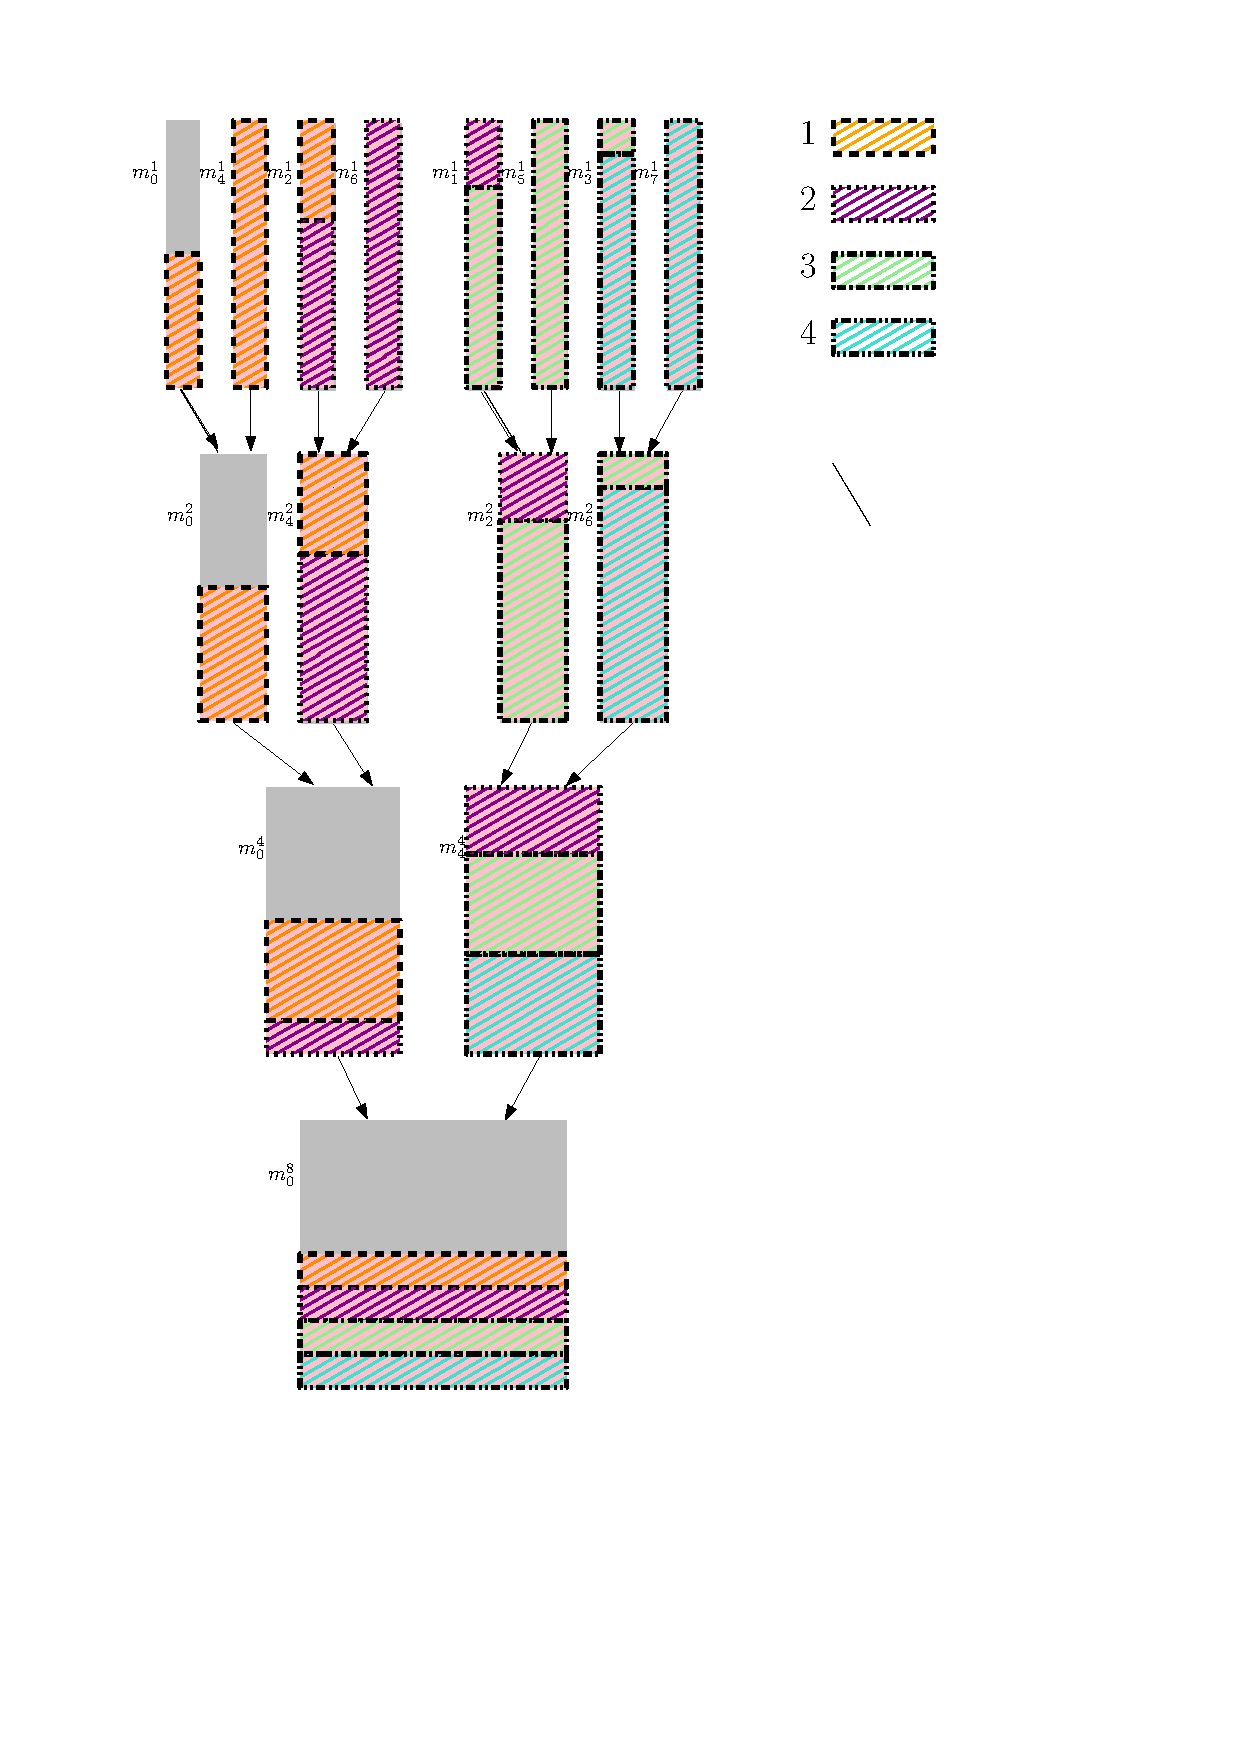
\includegraphics[height=\textheight-3cm]{processes_row_doublestep}
	\caption{Column Doublestep performed by 4 processes. The color in each step shows, which section gets performed by which process. $N=8$, $\omega = 2$, $rank=2$, $\lambda=4$.}
	\label{fig::colum_DS_distribution}
\end{figure}

\begin{algorithm} [H]
	\begin{algorithmic}[1]
		\State $\delta = \frac{lines.size}{\lambda}$
		\State $D=2^{step}$
		\For{$i \leftarrow 0$ to $\delta$}
				\State $(l,si) = lines[\delta\cdot key+i]$
				\If {$l < \frac{D}{2}$}
					\State $m_{si}^{D}[l] \leftarrow m_{\frac{si}{2}}^\frac{D}{2}[l]+m_{\frac{si+N}{2}\%N}^\frac{D}{2}[l]$
				\Else
					\State $m_{si}^{D}[l] \leftarrow m_{\frac{si}{2}}^\frac{D}{2}[(l+\frac{si}{2})\%N]+m_{\frac{si+N}{2}\%N}^\frac{D}{2}[(l+\frac{si+N}{2})\%]$
				\EndIf
		\EndFor
	\end{algorithmic}
\caption{StepOfColumnDoublestep($N,step,lines,\lambda , key$)}
\label{code::DS_Per}
\end{algorithm}

To update the image-matrix-slice, the processes need to add the final shift-matrix $m_0^N$. We can again distribute the rows to the different processes evenly, as we did with parallel Doublestep. The only difference is that there is just one shift-matrix to add. How to update the image matrix for Perpendicular Doublestep is shown in Algorithm \ref{code::DS_Per_im}. The $key\in \{0,1,\ldots,\omega-1\}$ refers to the machine.\\




\begin{algorithm}
	\begin{algorithmic}[1]
		\State $\Delta = \frac{N}{\omega}$
		\State $\delta = \frac{ \Delta}{\lambda}$
		\For{$l \leftarrow \delta\cdot indicesank$ to $\delta\cdot (indicesank+1)$}
			\State $I_t \leftarrow I_t[\Delta+l]+m_0^N[\Delta+l]$
		\EndFor
	\end{algorithmic}
\caption{UpdateImagePerpendicular($N,m_0^N,  \lambda ,indicesank$)}\label{euclid}
\label{code::DS_Per_im}
\end{algorithm}

\subsubsection{Complexity}
\label{sec::MultiProsComplex}
Since Multiprocessing Doublestep consists of a row- and a column part, we will discuss the complexity of these two parts separately.\\

The relevant parts of the complexity of MPIFT with dictionaries and row-Doublestep have been discussed before. Calculating a full row-shift dictionary takes
\[
\frac{N\cdot \beta}{\lambda}
\] complex multiplication per kernel and 
\[ \frac{(\beta-N)\cdot N}{\lambda}
\] complex multiplication per kernel.
Doublestep takes $N^2$ complex additions per step, as seen in Section \ref{sec::DB_complexity}. For row-Doublestep, we only perform $\log{\frac{N}{\omega}}$ steps, so it requires 
\[
\log{\frac{N}{\omega}}\cdot N^2 
\] complex additions.
Calculating the image-matrix-slice means adding $\omega$ $\frac{N}{\omega}\times N$ matrices to the image matrix. This takes 
\[
\omega\cdot \frac{N}{\omega}\cdot N=N^2
\] complex additions.\\ 


For MPIFT with dictionaries and column-Doublestep the calculations are more complicated. Equation \eqref{calc::valuesShiftDicPerpendicular} shows how many values are needed in the column-shift-dictionary. Unless $\omega=1$ this is smaller than $N^2$, but for small $\omega$ it's asymptotic complexity still is $N^2$. So we need \[
\mathcal{O}(\beta\cdot N^2) 
\]complex additions and multiplications.

%steps to calculate per-shift-dic
\begin{equation}
\begin{split} 
N^2-N\cdot \omega-\frac{N}{\omega}+\frac{2(\omega^2-1)}{3\cdot \omega}
\end{split}
\label{calc::valuesShiftDicPerpendicular}
\end{equation}

Equation \eqref{calc::additions_in_per} shows how many complex additions are needed for column-Doublestpe. Like row-Doublestep, this has an asymptotic complexity of \[
\mathcal{O}(N^2\cdot \log{N})
\] complex addtions.




\begin{equation}
\begin{split} 
2\cdot \frac{N}{\omega}\cdot (N-1) - \frac{4\cdot (\frac{N}{\omega}-1)((\frac{N}{\omega})^2-N^2)}{3\cdot \frac{N}{\omega}} +\\
 \frac{2}{3}\cdot (2\cdot {(\frac{N}{\omega})}^2-3\cdot \frac{N^2}{\omega}+N^2) -2\cdot N^2\cdot \frac{N-\omega}{N}+N^2\cdot (n-\log(\omega))
 \end{split}
 \label{calc::additions_in_per}
\end{equation}

MPIFT with dictionaries and Doublestep gets performed by $\lambda$ processes working together. In the row case, it is guaranteed, that every step is neatly dividable by $\lambda$, Column-Doublestep can't guarantee this. Since we divide it as evenly as possible in the perpendicular case, we still get  
\[
\mathcal{O}(\frac{ \log{(N)}\cdot N^2}{\lambda})
\] complex additions for both cases. 


\subsection{Comparing}
\label{sec::Comparing}
In this section, we will compare, how efficient the three algorithms naive NPIFT, NPIFT with dictionaries and NPIFT with dictionaries and Doublestep are. Table \ref{fig::comparing} shows how many complex multiplications and complex addition these different approaches take. Since the differences are big enough, we will use the asymptotic complexity to compare. The amount of machines $\omega$ is not expected to be big, so we will assume $\omega=1$ for these comparisons. \\

Both approaches that use shift-dictionaries do a lot better when it comes to complex additions. This has nothing to do with the shift-dictionaries themselves, and only with the fact that they use shared memory, and can therefore distribute all the shift-vector calculations over multiple machines.

The only case where naive MPIFT has less complex additions is when $\beta \leq N$. In all other cases, MPIFT with dictionaries and Doublestep has the fastest asymptotic complexity, when it comes to complex additions. If $\beta < N^2$, the asymptotic complexity for MPIFT with dictionary is the same as naive MPIFT, regardless of the distribution of processes. 

\begin{figure} [H]
	\begin{center}
		\begin{tabular}{||c c c||} 
			\hline
			MPIFT Algorithm & complex multiplications & complex additions \\ [0.5ex] 
			\hline\hline
			naive & $\mathcal{O}(\beta\cdot N)$ & $\mathcal{O}(\frac{\beta\cdot N^2}{\phi})$  \\ 
			\hline
			with dictionary & $\mathcal{O}(\frac{\beta\cdot N}{\lambda})$ & $\mathcal{O}(\frac{\beta\cdot N}{\lambda}+\frac{N^3}{\phi})$  \\
			\hline
			\shortstack{with dictionary \\textbf{and} Doublestep} & $\mathcal{O}(\frac{\beta\cdot N}{\lambda})$ &
			$\mathcal{O}(\frac{\beta\cdot N}{\lambda}+\frac{N^2\cdot \log{N}}{\lambda})$  \\ 
			\hline
		\end{tabular}
	\end{center}
\captionof{table}{Comparing theoretical asymptotic complexity of different MPIFT algorithms. All values are per process }
\label{fig::comparing}
\end{figure}

Table \ref{fig::comparing_ratio} shows the ratios for the three approaches regarding the same measurements. When using MPIFT with dictionary we can reduce the amount of complex additions needed by $\frac{\beta}{N}$. The improvement gets better when we additionally use Doublestep, which will further by $\frac{N}{\log{N}}$ to a total of $\frac{\beta}{\log{N}}$.

By using shift-dictionaries The amount of complex multiplications only gets reduced by $\lambda$. Additional using Doublestep doesn't impact it significantly. This means that the efficiency increase we get is dependent on the physical infrastructure available and does not scale with $N$. In cases where $\lambda$ is limited, we foresee a new computational bottleneck.

\begin{figure} [H]
\begin{center}
	\begin{tabular}{||c c c c||} 
		\hline
		\shortstack{MPIFT \\Algorithm 1} & \shortstack{MPIFT \\ Algorithm 2} & \shortstack{complex \\mulltiplication \\ ratio} & \shortstack{complex\\ additions\\ratio} \\ [0.5ex] 
		\hline\hline
		naive & with Dictionary & $\frac{\lambda}{1}$ & $\frac{\beta}{N}$ \\ 
		\hline
		naive & \shortstack{with dictionary \\and Doublestep} & $\frac{\lambda}{1}$ & $\frac{\beta}{\log{N}}$ \\
		\hline
		with Dictionary & \shortstack{with dictionary \\textbf{and} Doublestep} & $1$ & $\frac{N}{\log{N}}$ \\  
		\hline
	\end{tabular}
\end{center}
\captionof{table}{Comparing ratio of significant measures per Kernel between MPIFT-implementations. We assume $\beta << N^2.$}
\label{fig::comparing_ratio}
\end{figure}

\subsection{Experiment}
\label{sec::Experiment}

\subsubsection{Setup}
\label{sec::setup}

To test the three Algorithms, we implemented them in \emph{C++}, using MPI (\emph{Message Passing Interface}) to communicate between nodes and to enable shared memory. The paper from Saad et al. used Apache Flink. We did not use this, since Apache Flink doesn't offer possibilities so share local memory. We used the Open MPI library, that implements MPI for \emph{C++}.\\

We used two servers, provided by the institute for computer science of the University of Zurich. Each of them has 48 cores, and 188 GB of memory using Intel Xeon Silver 4214 Processors. In order to record the measured time, each implementation wrote to the file-system at fixed point in its program.

Naive MPIFT only recorded the total time elapsed to handle one batch. We did this, because the constant writing that would result from writing after each single visibility would slow down the system and the overall elapsed time would be less precise.  Also since naive MPIFT is the only one that handles visibilities one by one, we would have nothing to compare the time for a single visibility to.

For MPIFT with dictionary we measured the overall elapsed time, the time it took to calculate each dictionary and the time to run SPIFT on all values in all dictionaries. This way, we can compare the total time elapsed for the naive approach, and the time to calculate the dictionaries with MPIFT with dictionaries and Doublestep.

For MPIFT with dictionaries and Doublestep we measured the time to calculate each dictionary and the time it took to calculate row- and column-Doublestep. This way, we can see if the implementations bottleneck is more with column-Doublestep as we would expect. We can also compare the row- and shift-dictionary creation with the previous approach. We are calculating the row-dictionary the same way, so the times should be more or less the same. The column-dictionary is calculated differently, and it will be interesting to see if the times are significantly different.\\

We used a constant $N=2^{13}=8192$ for all experiments. We started by using two machines $\omega=2$ with $\lambda=16$ processes each. After that we varied the amount of processors per machine $\lambda=8,\lambda=32$. Initially we used a batch-size of $\beta=42642$. Later we also used $\beta=170568$ and $\beta=340992$, to confirm that only the calculation of the shift-dictionary and the whole of the naive approach would suffer under this.
 

\subsubsection{Result}
\label{sec::result}

Figure \ref{fig::compare_implementations_exp } shows how fast the three implementations were per batch. Naive MPIFT with a speed of 2'500  seconds was clearly the slowest. Already including shift-dictionaries made it almost three times as fast with an average of 890 seconds per batch. MPIFT with dictionaries and Doublestep took an average of $10.5$ seconds and was by far the fastest, 240 times faster than the naive approach and 80 times faster than the with only shift-dictionaries. 

\begin{figure}[H]
	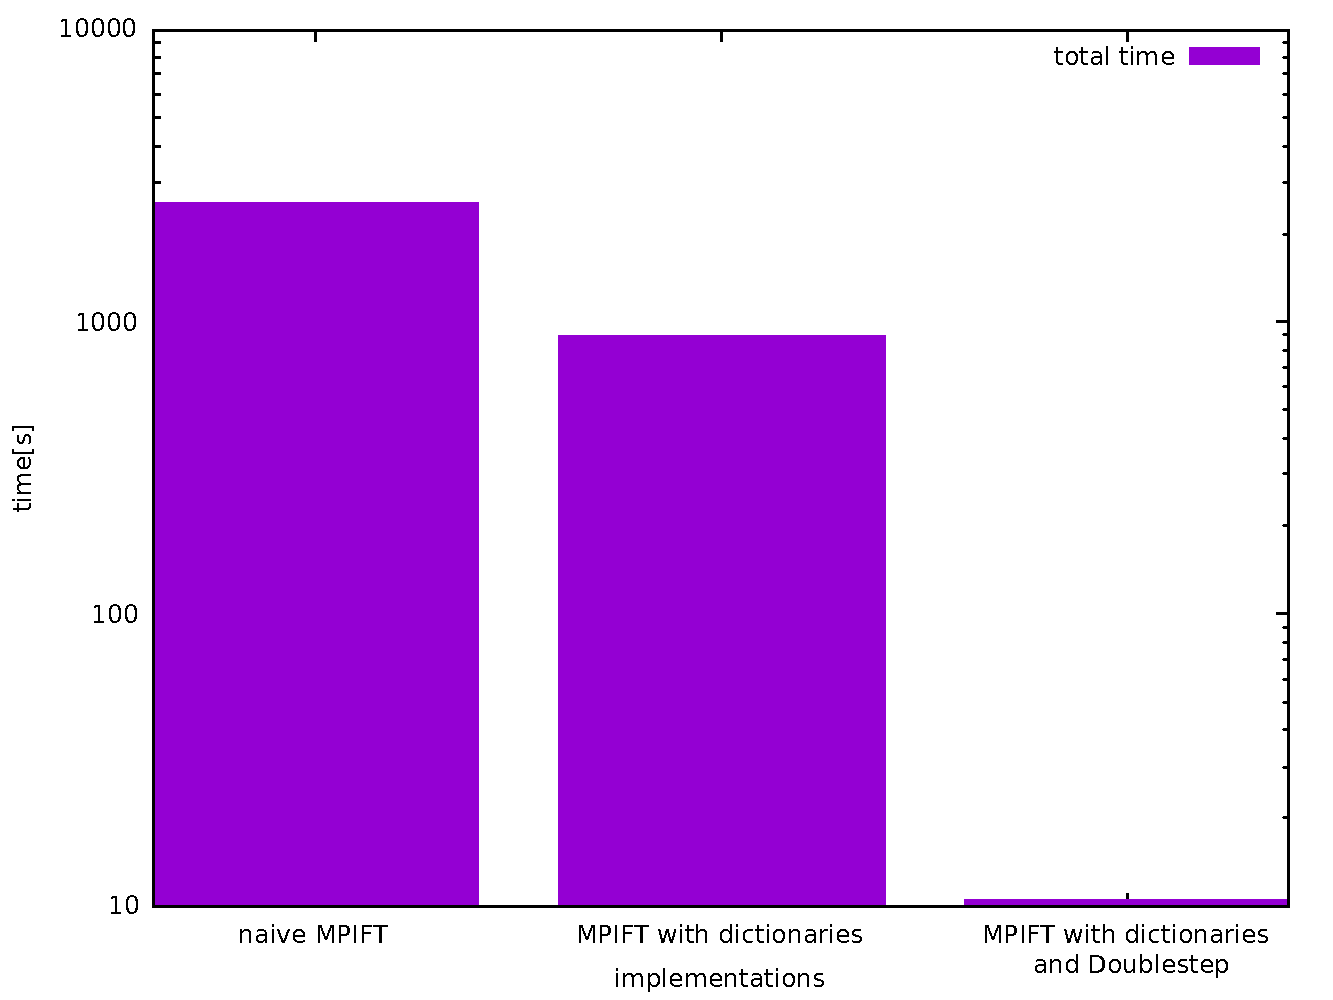
\includegraphics[width=380pt]{comp}
	\caption{Total time required by naive MPIFT, MPIFT with dictionaries and MPIFT with dictionaries and Doublestep
	\label{fig::compare_implementations_exp } with $N=8192$, $\phi=64$, $\omega=2$, $\lambda=32$, $\beta=42642$}
\end{figure}

Figure \ref{fig::compare_Spift_DS} compares the times that MPIFT with dictionaries and MPIFT with dictionaries and Doublestep need to update the image-matrix after having calculated the shift-dictionaries. With $1.7$ seconds, Doublestep is 90 times faster than SPIFT to add the row-shift-dictionary, and with $4.9$ seconds 55 times faster with the column-shift dictionary. Both row- and column-Doublestep have the same asymptotic complexity, but column-Doublestep requires more complex additions. This explains why the ratio for column-shift is smaller than for row-shift.

It is also of note that for MPIFT with dictionaries and Doublestep, row-shift is significantly faster than column shift. This is on one hand because column-Doublestep requires more complex additions, and on the other hand because column-Doublestep calculates more steps of Doublestep and therefore has a larger computational overhead. For MPIFT with dictionary, column-shift is also slower. This is because in our implementation, we iterated over the rows and then over the columns, leading to a loss because of poor memory access.

\begin{figure}[H]
	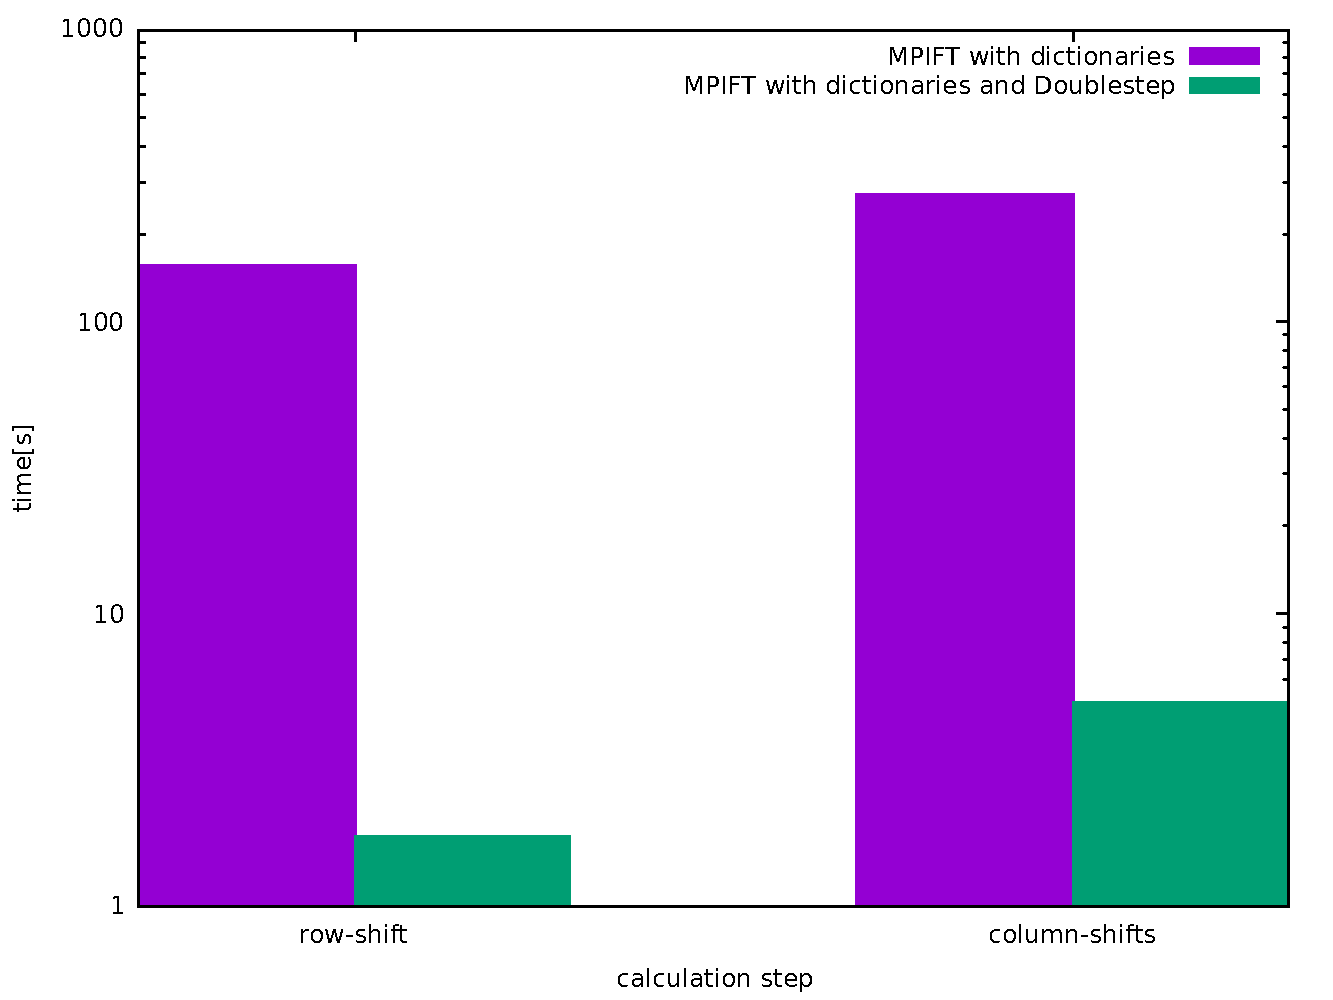
\includegraphics[width=380pt]{compare_with_Dic_to_DS_64}
	\caption{Time required to update the image matrix after having calculated the shift-dictionaries by MPIFT with dictionaries and Doublestep, $N=8192$, $\phi=64$, $\omega=2$, $\lambda=32$, $\beta=42642$}
	\label{fig::compare_Spift_DS}
\end{figure}

Figure \ref{fig::compare_kernels_DS} shows a breakdown of the times for MPIFT with dictionaries and Doublestep for different degrees of parallelism $\lambda\in\{8,16,32\}$. When the amount of kernel increases, the computational time goes down, but it doesn't go down as much as hoped. The amount of complex additions is halved when the amount of processes is doubled. We expected that the time for row- and column-Doublestep would be close to halved, but we don't see that. We assume this is because we implemented Doublestep without any optimizations for multi-threading. So threads are created and destroyed more often than needed, leading to an increased overhead that gets very noticeable when times get as low as they are here.

\begin{figure}[H]
	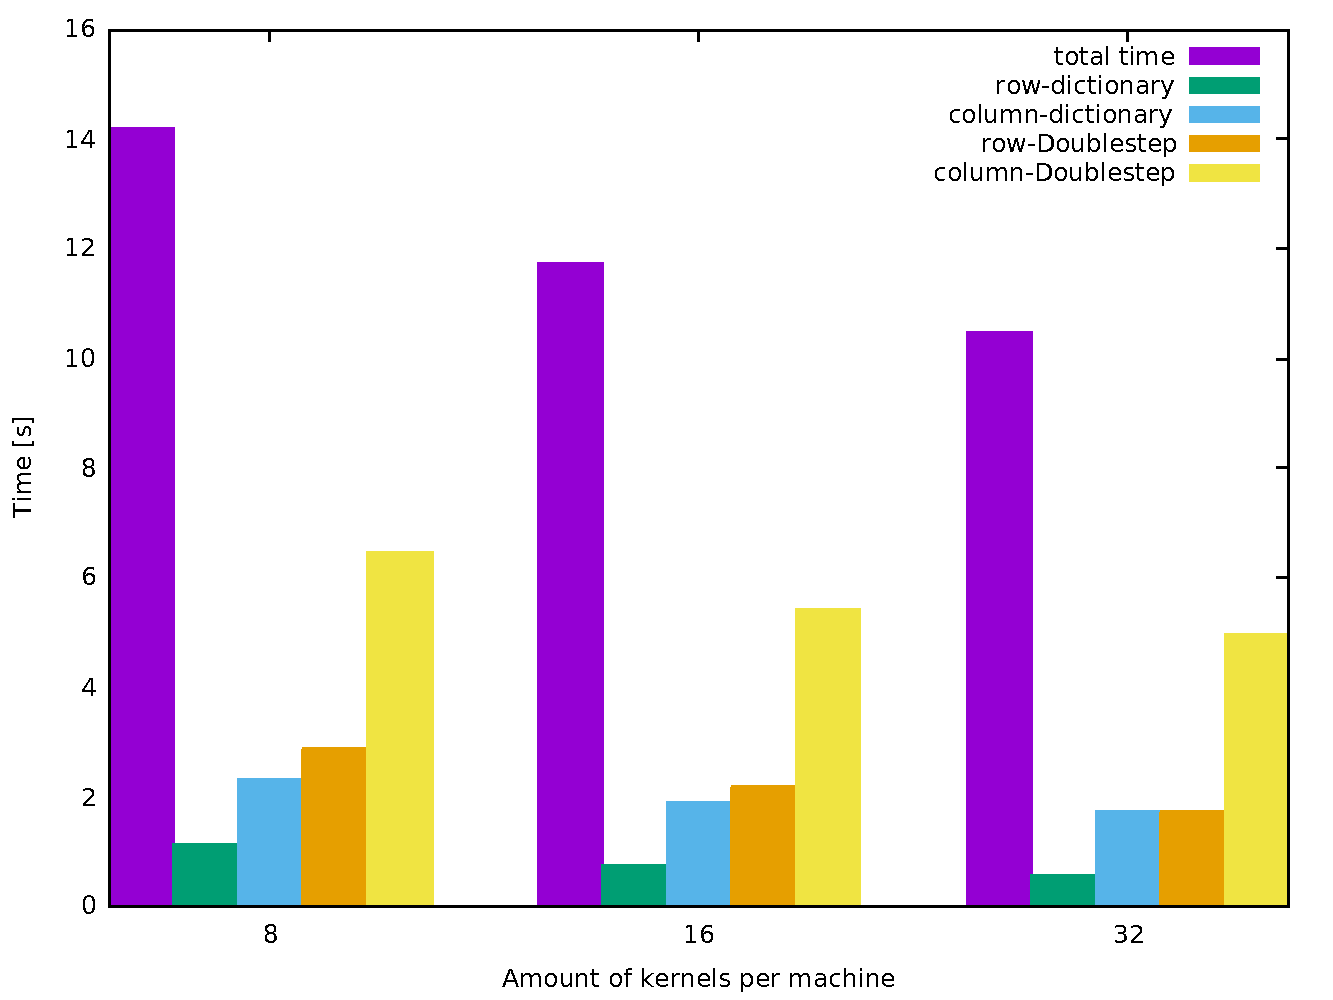
\includegraphics[width=380pt]{Doublestep_different_amount_of_kernels}
	\caption{Breakdown of MPIFT with dictionaries and Doublestep with varying amounts of local processes $\lambda$, $N=8192, \beta=42642$}
	\label{fig::compare_kernels_DS}
\end{figure}

Figure \ref{fig::compare_batchsize_DS} shows how Doublestep deals with different batch-sizes
\[
\beta \in \{43643,170568,340992\}.
\]
 As expected, the time for row- and column-Doublestep do not change. This is because they work only on shift-dictionaries and not directly on the batch.

We also see for the parallel dictionary that the jump between $\beta = 42642$ to $\beta=170568$ is bigger than from $\beta=170568$ to $\beta=340992$. This is because for smaller batch-sizes, there are still shift-indices that only have one visibility, therefore saving on complex additions. When the batch sizes increases, this effect becomes increasingly unlikely.

We also see that calculating the column-shift-dictionary takes significantly longer than the row-dictionary. When calculating the column-shift-dictionary, we only calculated the rows for each shift-vector, that were needed to perform column-Doublestep. This decreases the amount of complex operations needed to compute the shift-dictionary, but again at the cost of computational overhead. This is why initially the difference between row- and column-dictionary computation is big, but decreases when the batch-size increases, since the saved operations become more important than the computational overhead. But the column-shift dictionary only has half as many visibilities and is even for bigger batch-sizes only as efficient as calculating the row-shift dictionary. This is an indication that the optimization here is not worth the effort and it would be faster to simply compute the full shift-dictionary as normal.


\begin{figure}[h]
	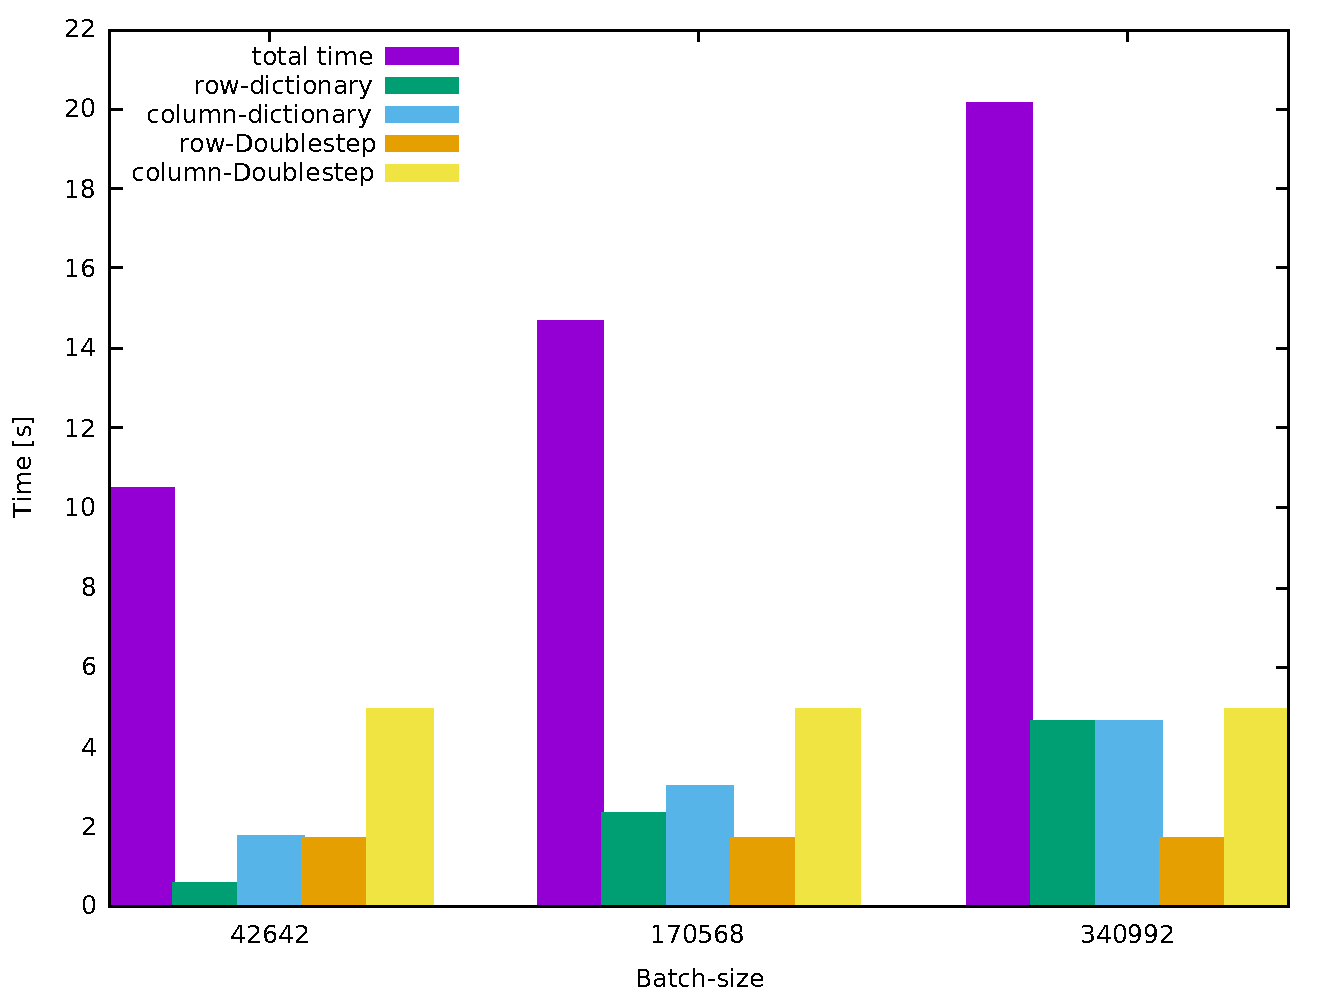
\includegraphics[width=380pt]{compare_ds_batchsize}
	\caption{Breakdown of MPIFT with dictionaries and Doublestep with varying batch size   $\beta$, $N=8192, \phi=64$.}
	\label{fig::compare_batchsize_DS}
\end{figure}


\newpage
\section{Conclusion}
\label{sec::conclusion}
MPIFT with dictionaries and Doublestep is significantly faster than the naive approach or only using dictionaries, both in theory and in an experimental setting. We couldn't reach the full theoretical improvement of $\mathcal{O}(\frac{N}{\log N})$ in an experimental setting. Presumably this is because of the computational overhead our implementation of Doublestep introduced. MPIFT with dictionaries and Doublestep scales better than both other MPIFT variants.

With Doublestep, updating the image-matrix becomes more efficient and the amount of complex additions is reduced. Introducing a shift-dictionary can further reduce the amount of complex additions. But neither of these methods can reduce the amount of complex multiplications significantly. The creation of the shift-dictionary and the complex multiplications needed for it become the new computational bottleneck.\\

Since this report build on the work of Saad et al. \cite{spift}, its main focus are applications in radio-astronomy. But as with SPIFT, Doublestep could proof useful in other fields that use Discrete Fourier Transformation as well.

Further research could go into increasing the efficiency of Doublestep by reducing the computational overhead and optimizing threading. Since Doublestep mostly requires complex additions and shared memory it could be a worthwhile endeavor to analyze if it runs efficiently on a graphic card.  

\pagebreak

\bibliography{ref}

\pagebreak

\section{Appendix}

The complete source code used for testing is accessible on \emph{Github} at https://github.com/degenwitz/SPIFT\_Thesis.

\end{document}
